\documentclass[11pt]{article}
\usepackage[T1]{fontenc}
\usepackage[utf8]{inputenc}
\usepackage{lmodern}
\usepackage[margin=1in]{geometry}
\usepackage{microtype}
\usepackage{float}
\usepackage{tikz}
\usepackage[section]{placeins}
\usepackage{amsmath}
\usepackage{array}
\usepackage{booktabs}
\usepackage{url}
\usepackage[hidelinks]{hyperref}

\newcommand{\doi}[1]{\href{https://doi.org/#1}{\nolinkurl{doi:#1}}}
% Generated by paper/tools/gen-numbers.mjs from paper/data/results.json. Do not edit.
\newcommand{\rustRuns}{10}
\newcommand{\jsRuns}{10}
\newcommand{\nodeVersion}{25.2.0}
\newcommand{\rustcVersion}{1.99.1}
\newcommand{\veeEightVersion}{14.1.146.11}
\newcommand{\cpuName}{12th Gen Intel Core i5-1235U}
\newcommand{\memoryGb}{16}
\newcommand{\osName}{Windows 10 Pro 10.0.19045}
\newcommand{\clauseCount}{15}
\newcommand{\ablationCount}{14}
\newcommand{\exhaustiveStatesA}{44{,}493}
\newcommand{\exhaustiveStatesB}{78{,}348}
\newcommand{\quantTests}{75}
\newcommand{\repositoryTests}{76}
\newcommand{\alienCorpus}{198}
\newcommand{\alienPrograms}{4{,}000}
\newcommand{\alienPortDiffer}{49}
\newcommand{\alienReverseValidate}{1{,}589}
\newcommand{\alienForbidParallel}{231}
\newcommand{\alienNoTail}{63}
\newcommand{\alienMoveBothAxes}{7}
\newcommand{\alienFlatFrozen}{0}
\newcommand{\alienFlatPassed}{198}
\newcommand{\polyfillCorpus}{39}
\newcommand{\polyfillPrograms}{3{,}000}
\newcommand{\polyfillPortHookThrow}{57}
\newcommand{\polyfillRetainHookThrow}{9}
\newcommand{\polyfillStableEraseOrder}{9}
\newcommand{\polyfillRetainInactive}{39}
\newcommand{\polyfillRetainPhysical}{59}
\newcommand{\polyfillRetainFlips}{13}
\newcommand{\wpfSnapshotCopiesA}{4{,}490}
\newcommand{\wpfSnapshotCopiesB}{4{,}452}
\newcommand{\wpfCowCopiesA}{511}
\newcommand{\wpfCowCopiesB}{363}
\newcommand{\wpfSnapshotFactorA}{8.8}
\newcommand{\wpfSnapshotFactorB}{12.3}
\newcommand{\wpfRetiredProgramsA}{11}
\newcommand{\wpfRetiredProgramsB}{4}
\newcommand{\wpfDirectedTotal}{28}
\newcommand{\wpfGenerated}{3{,}000}
\newcommand{\wpfRandom}{6{,}000}
\newcommand{\wpfNextDirected}{27}
\newcommand{\salsaReverseGenerated}{657}
\newcommand{\salsaReverseHoldout}{667}
\newcommand{\salsaReverseFresh}{672}
\newcommand{\salsaReversePercent}{22}
\newcommand{\salsaReverseDirected}{3}
\newcommand{\salsaReverseValues}{0}
\newcommand{\salsaStoreEventsPerExecution}{2.56}
\newcommand{\salsaTotalPrograms}{9{,}019}
\newcommand{\reorderReuseMutations}{425}
\newcommand{\stableReuseMutations}{25}
\newcommand{\reorderOverStable}{17}
\newcommand{\salsaPackedBytes}{28.8}
\newcommand{\salsaSplitBytes}{61.1}
\newcommand{\salsaAosBytes}{85.2}
\newcommand{\salsaDensityRatio}{2.1}
\newcommand{\salsaPackedNs}{48.0}
\newcommand{\salsaPackedNsMin}{45.0}
\newcommand{\salsaPackedNsMax}{49.3}
\newcommand{\salsaSplitNs}{54.7}
\newcommand{\salsaAosNs}{53.0}
\newcommand{\salsaAosCursorNs}{76.7}
\newcommand{\salsaIntrusiveCursorNs}{81.1}
\newcommand{\salsaHashNs}{132}
\newcommand{\wpfCowNs}{36.6}
\newcommand{\wpfIntrusiveNs}{64.7}
\newcommand{\wpfAosNs}{65.7}
\newcommand{\wpfSoaNs}{122}
\newcommand{\wpfCowRatio}{1.8}
\newcommand{\salsaCowlessGain}{1.11}
\newcommand{\rustQuantRatio}{1.19}
\newcommand{\jsQuantRatio}{1.42}
\newcommand{\jsOverRustQuant}{3.34}
\newcommand{\rustCalmRatio}{2.73}
\newcommand{\jsCalmRatio}{3.42}
\newcommand{\jsOverRustCalm}{2.45}
\newcommand{\rustChurnRatio}{3.66}
\newcommand{\jsChurnRatio}{4.71}
\newcommand{\jsOverRustChurn}{2.22}
\newcommand{\jsRatioMin}{1.42}
\newcommand{\jsRatioMax}{4.71}
\newcommand{\rustRatioMin}{1.19}
\newcommand{\rustRatioMax}{3.66}
\newcommand{\jsOverRustMin}{2.22}
\newcommand{\jsOverRustMax}{3.34}
\newcommand{\boundaryFieldNs}{2.20}
\newcommand{\boundaryWeakNs}{23.7}
\newcommand{\boundaryRatio}{11}
\newcommand{\crossCells}{60}
\newcommand{\crossContiguousBest}{60}
\newcommand{\crossPackedLosses}{3}
\newcommand{\crossInplaceLosses}{0}
\newcommand{\crossPackedRatioMin}{0.12}
\newcommand{\crossPackedRatioMax}{17.9}
\newcommand{\crossPackedRatioMedian}{9.00}
\newcommand{\crossInplaceRatioMin}{1.64}
\newcommand{\crossInplaceRatioMax}{30.0}
\newcommand{\crossInplaceRatioMedian}{23.4}
\newcommand{\crossPackedLossCells}{$N=8$, $S=0.9$, none; $N=8$, $S=1$, none; $N=64$, $S=1$, none}
\newcommand{\crossInplaceLossCells}{none}
\newcommand{\stableEightPacked}{6.81}
\newcommand{\stableEightInplace}{0.482}
\newcommand{\stableEightCursor}{1.01}
\newcommand{\stableFiveTwelvePacked}{0.772}
\newcommand{\stableFiveTwelveInplace}{0.437}
\newcommand{\stableFiveTwelveCursor}{1.54}
\newcommand{\stableBigPacked}{0.883}
\newcommand{\stableBigInplace}{0.458}
\newcommand{\stableBigCursor}{2.34}
\newcommand{\chaoticFiveTwelveCursor}{49.3}
\newcommand{\noneFiveTwelveCursor}{1.54}
\newcommand{\crossCursorBestEight}{0.790}
\newcommand{\aosRebuildCostMin}{12.0}
\newcommand{\aosRebuildCostMax}{16.3}
\newcommand{\crossTailBeatsCursor}{58}
\newcommand{\crossMaxLinkedAdvantage}{8.6}
\newcommand{\noiseSeries}{29}
\newcommand{\noisePinnedMedian}{1.14}
\newcommand{\noisePinnedMax}{1.68}
\newcommand{\noiseUnpinnedMedian}{1.72}
\newcommand{\noiseUnpinnedMax}{3.41}
\newcommand{\noiseUnpinnedRuns}{5}
\newcommand{\gcScenarios}{11}
\newcommand{\gcRounds}{20}
\newcommand{\gcAllHeld}{all}
\newcommand{\observerTurns}{4{,}000}
\newcommand{\observerTrials}{10}
\newcommand{\observerEveryOneCleared}{0}
\newcommand{\observerEveryOneMajors}{13}
\newcommand{\observerEveryTwoCleared}{2}
\newcommand{\observerEveryTenCleared}{5}
\newcommand{\observerEveryHundredCleared}{10}
\newcommand{\observerEarlierEveryTwo}{0}
\newcommand{\observerEarlierEveryTen}{8}
\newcommand{\observerEverySlowCleared}{10}

\newcommand{\figlevel}[3]{\node[draw,text width=3.5cm,minimum height=1.3cm,align=center,font=\footnotesize\bfseries] at (0,-#1*1.75) {#2}; \node[text width=10.4cm,anchor=west,font=\footnotesize] at (2.3,-#1*1.75) {#3};}
\newcommand{\figarrow}[1]{\draw[->] (0,-#1*1.75-0.68) -- (0,-#1*1.75-1.07);}

\title{The Cost of Reactive Graph Abstractions:\\ An Experimental Study of Semantics, Topology, and Memory Layout}
\author{Andrii Volynets}
\date{November 2026}

\begin{document}
\maketitle

\begin{abstract}
Reactive libraries, build systems and query engines all maintain dependency relations between computations, and an effort to standardize signals in JavaScript proposes to specify that graph at the language level. We investigate whether reactive graph topology requires runtime-level primitives by constructing semantically equivalent implementations with alternative memory layouts and measuring their behavior across JavaScript and Rust. We state a candidate primitive, a store of ordered bidirectional relations with stable identity and walk-safe retirement, as an executable contract of \clauseCount{} clauses, and test which clauses five systems need: Quant, Alien Signals, the TC39 signal polyfill, WPF weak events and Salsa. No tested behaviour required a runtime-provided store, and Alien, WPF and Salsa ran with all relational state in the client. Physically, the systems divide into trace-shaped and graph-shaped workloads that favour different layouts. On the three large graph tapes, dense integer-indexed slots beat pointer-joined records by median factors of \rustRatioMin{} to \rustRatioMax{} in Rust and \jsRatioMin{} to \jsRatioMax{} in plain JavaScript over typed arrays, which stayed \jsOverRustMin{} to \jsOverRustMax{} times slower than Rust. Standard weak-reference APIs sufficed in all \gcScenarios{} collector scenarios on V8. Rebuilt on dense slots, Alien Signals preserved behaviour on \mSixPrograms{} differential programs, but end to end its time was indistinguishable from the original on an application-shaped workload and worse on propagation and graph creation, and its integer-named relations were invisible to the collector. The logical relation survived abstraction; no universal physical graph emerged. We found no layout advantage requiring VM ownership in these single-threaded workloads; collector-visible dense relations are the one capability plain JavaScript did not provide. We built no native implementation. We do not propose a replacement signal API.
\end{abstract}

\section{Introduction}

Every incremental system keeps a record of what depended on what. Attribute evaluators \cite{demers1981,hudson1991}, function caches \cite{pugh1989}, self-adjusting programs \cite{acar2006}, build systems \cite{erdweg2015,mokhov2020}, reactive user interfaces \cite{elliott1997,cooper2006,czaplicki2013,bainomugisha2013} and compiler query engines \cite{salsa} differ in almost everything else, yet each maintains relational state between computations and updates it as those computations run again.

In JavaScript these structures have started to look alike. Vue moved its reactivity core to ``a doubly-linked list data structure inspired by'' Preact Signals \cite{vue10397,preactsignals}, and Alien Signals \cite{aliensignals} is built from the same kind of link records. The TC39 Signals proposal, at Stage~1, targets ``the precise core semantics of the underlying signal graph'' and reports: ``It turns out that existing Signal libraries are not all that different from each other, at their core.'' \cite{tc39signals}. One reading of this convergence is that a single structure is being reinvented, and that a language runtime is a natural home for it.

This paper tests that reading experimentally. We investigate whether reactive graph topology requires runtime-level primitives by constructing semantically equivalent implementations with alternative memory layouts and measuring their behavior across JavaScript and Rust.

Discussions of the topic tend to merge three questions, and we keep them apart. Which relational capabilities does a system use, and which does it observably require? Where must those capabilities be held for its behaviour to be preserved? Which physical layout implements them well? A positive answer to the first says nothing about the second, and an answer to the second says little about the third.

We pose four research questions.

\begin{description}
\item[RQ1.] Which relational capabilities do real incremental systems use, and which are observably required?
\item[RQ2.] Must any of those capabilities live in a runtime-provided store for behaviour to be preserved?
\item[RQ3.] Which memory layouts do these workloads favour, and does the best layout's advantage require leaving the host language?
\item[RQ4.] Does a production collector with standard weak-reference APIs leave any tested lifecycle property unattainable?
\end{description}

\paragraph{Contributions.}
\begin{itemize}
\item An executable contract for a candidate relation primitive (\clauseCount{} clauses) together with \ablationCount{} single-mechanism ablations, each with a shortest witness history. The candidate is treated as guilty until required: a mechanism stays only if some client needs it.
\item A client-minimality study of five systems, Quant, Alien Signals, the TC39 signal polyfill, WPF weak events and Salsa, using ports, one-at-a-time ablations and differential testing. WPF and Salsa are judged by their own executables, not by our translations of them.
\item A physical study over operation tapes recorded from those clients. It compares contiguous, pointer-joined and dense indexed layouts in Rust and in plain JavaScript, and it includes a grid comparing ten rebuild and reuse strategies.
\item An end-to-end control: an independent signal runtime rebuilt on dense slots under a protocol fixed in advance, judged by its own tests, by differential search and by a retention probe.
\item A feasibility study of lifecycle properties under a production collector, including a measured observer effect of \texttt{WeakRef} polling.
\end{itemize}

\paragraph{Summary of findings.}
No tested behaviour required a runtime-provided store, so behaviour identifies required capabilities and not their substrate. Alien, WPF and Salsa were also run with all their relational state in the client (Table~\ref{tab:capabilities}). Figure~\ref{fig:levels} shows the levels of the argument. Observable semantics constrains capabilities and cannot establish who owns the substrate: the candidate did not show semantic necessity, which does not reject it as a primitive, since almost any primitive can be emulated. Physically, the systems fall into two families that favour different layouts. The advantage of dense layouts on graph-shaped work reproduces in plain JavaScript over typed arrays. On the studied workloads and implementations we found no layout advantage that required ownership by the virtual machine. Inside a complete runtime the same layout reduced memory and collector work but gave no general gain in time, and it cost something replay cannot show: relations named by integers are invisible to the collector.

These findings are bounded. We measured single-threaded workloads on one machine and one JavaScript engine, we did not build a store inside a VM, and we did not study interoperability between libraries. Section~\ref{sec:threats} states the limits and Section~\ref{sec:implications} separates what the results bear on from what they do not. We do not propose a replacement signal API.

\begin{figure}[tbp]
\centering
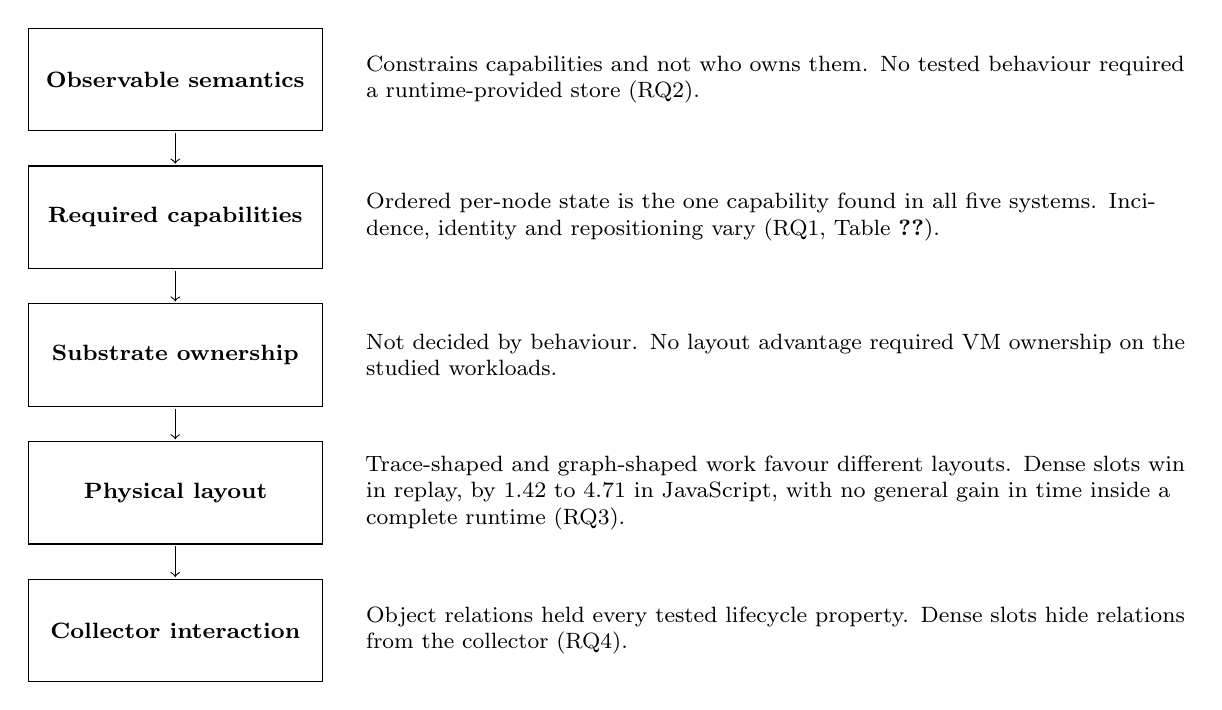
\begin{tikzpicture}
\figlevel{0}{Observable semantics}{Constrains capabilities and not who owns them. No tested behaviour required a runtime-provided store (RQ2).}
\figarrow{0}
\figlevel{1}{Required capabilities}{Ordered per-node state is the one capability found in all five systems. Incidence, identity and repositioning vary (RQ1, Table~\ref{tab:capabilities}).}
\figarrow{1}
\figlevel{2}{Substrate ownership}{Not decided by behaviour. No layout advantage required VM ownership on the studied workloads.}
\figarrow{2}
\figlevel{3}{Physical layout}{Trace-shaped and graph-shaped work favour different layouts. Dense slots win in replay, by \jsRatioMin{} to \jsRatioMax{} in JavaScript, with no general gain in time inside a complete runtime (RQ3).}
\figarrow{3}
\figlevel{4}{Collector interaction}{Object relations held every tested lifecycle property. Dense slots hide relations from the collector (RQ4).}
\end{tikzpicture}
\caption{The levels of the argument and what the study found at each. An answer at one level does not follow from the level before it.}
\label{fig:levels}
\end{figure}

\section{Background}
\label{sec:background}

\subsection{Dependency state in incremental systems}

We call the computation that depends the \emph{consumer} and what it depends on the \emph{producer}. A relation connects the two. Reading a relation from consumer to producer serves validation, the question of whether anything a computation used has changed. Reading it from producer to consumer serves propagation, the question of who must be told about a change.

Systems store these relations in different forms. Self-adjusting computation represents an execution as a dynamic dependence graph with timestamps \cite{acar2006,acar2009}, using order maintenance \cite{dietz1987}. Adapton keeps demanded computations and their edges in a demanded computation graph \cite{hammer2014}, and later work uses first-class names to identify computations to be reused across differing runs \cite{hammer2015}. Mokhov et al.\ describe build systems through their traces, where a verifying trace records each key's dependencies, and observe of one scheme that ``actual build steps are performed as a consequence of checking'' whether a key needs rebuilding \cite{mokhov2020}. Signal libraries combine an eager notification pass with lazy pulling of values, a combination also studied as push-pull reactive programming \cite{elliott2009}.

\subsection{The TC39 Signals proposal}

The proposal \cite{tc39signals} and its polyfill \cite{signalpolyfill} define state signals, computed signals and watchers. We use the text at commit \texttt{9124ed9} and the polyfill at \texttt{fba09f8}, and we keep them as separate evidence layers, because they differ. The proposal says it is ``providing interoperability through common signal graph and auto-tracking mechanism''. On performance it is modest: ``We suspect that native C++ implementations of Signal-related data structures and algorithms can be slightly more efficient than what is achievable in JS, by a constant factor.'', and ``no algorithmic changes are anticipated''. It also states a condition for its own advance, that signals ``provide real benefits over framework-provided signals''. In the proposal's issue tracker, one participant triaging a request preferred that applications end up with ``a single, internal, Signals graph'' \cite{tc39issue259}, and another request asks for the graph protocol to be exposed \cite{tc39issue258}.

\subsection{Memory layout}

Pointer-joined records are the conventional form of a dynamic graph in a managed language. The alternatives have a long history outside this domain: structure splitting and field reordering \cite{chilimbi1999b}, cache-conscious placement \cite{chilimbi1999}, segregation of data structures into pools \cite{lattner2005}, vertical partitioning inside a storage page \cite{ailamaki2001}, and adjacency representations for static and streaming graphs \cite{shun2013,dhulipala2019,grinten2022}. In a dense layout, a relation is an integer index, and its fields sit in one array of structures (AoS) or several parallel arrays (SoA). JavaScript offers this through typed arrays, at the price that an array holds numbers and cannot hold references to objects.

\subsection{Weak references in ECMAScript}

ECMAScript provides \texttt{WeakRef}, \texttt{FinalizationRegistry} and \texttt{WeakMap} \cite{ecma262}. It promises no collection. A \texttt{WeakRef} target that was created or dereferenced during a job is kept to the end of that job, and neither the clearing of that list nor finalization ``may interrupt synchronous ECMAScript execution''. A \texttt{WeakMap} behaves as an ephemeron table \cite{hayes1997}. Formal treatments of weak references \cite{donnelly2006} and the difficulties of finalization \cite{boehm2003} predate these APIs.

\section{Study design}
\label{sec:design}

\subsection{Three kinds of minimality}

We distinguish three questions about a candidate primitive and settle them with different evidence.

\begin{description}
\item[Contract minimality.] Given the clauses, which mechanisms do they need? Settled by ablating the abstract machine.
\item[Client minimality.] Which clauses do real clients need? Settled by ports, ablations and differential testing.
\item[Physical minimality.] Which representation implements what survives, at what cost? Settled by measurement.
\end{description}

The inclusion rule is strict: a mechanism enters the candidate only if a clause breaks without it, or if a port cannot keep its observable semantics without it. That other runtimes have a mechanism, or that it is convenient, does not count.

\subsection{The candidate}

The candidate, called L0 below, is an abstract machine rather than an API. A relation $e=(u,v)$ sits in exactly two ordered lists, $L(u)$ and $R(v)$. Nodes and relations are named by handles of slot and generation, and a handle's status only moves forward, from live to retired to stale. Each direction declares its retention at creation, and liveness is the least fixed point of reachability from explicit roots along retaining directions. Operations are \texttt{relate}, \texttt{unlink}, \texttt{moveAfter}, \texttt{first}, \texttt{next}, immutable endpoint and retention readers, one 32-bit metadata word, epoch \texttt{enter} and \texttt{exit}, and an explicit \texttt{collect}.

The \clauseCount{} clauses cover stable identity, dual incidence, order, permutation, reachability, GC transparency, deferred reuse, walk continuation, metadata, multiplicity, failure atomicity, lifecycle, semantic opacity, the absence of callbacks, and local complexity. Each of \ablationCount{} ablations removes one mechanism and yields a shortest history on which a clause breaks, within a bound of 12 operations (Table~\ref{tab:ablations}). Semantic opacity and the absence of callbacks hold by construction, and local complexity is a bound that the model cannot exercise, so these three clauses have no witness. The reference machine and two controls are checked exhaustively within small bounds (\exhaustiveStatesA{} and \exhaustiveStatesB{} states). The reference machine is array-backed on purpose, so it cannot test the local-complexity clause; the physical study addresses layouts but does not verify that clause as a bound.

\begin{table}[tbp]
\centering
\scriptsize
% Generated by paper/tools/gen-numbers.mjs. Do not edit.
\begin{tabular}{l p{4.2cm} l p{2.4cm} p{6.2cm}}
\toprule
Ablation & Removes & Kind & Clauses broken & Shortest witness \\
\midrule
\texttt{no-generation} & generation guard on handles & safety & identity & \texttt{n0=node; collect; n1=node} \\
\texttt{one-bit-generation} & unbounded generation (wraps at 2 reuses) & safety & identity & \texttt{n0=node; e0=relate(n0,n0,strong); unlink(e0); e1=relate(n0,n0,strong); unlink(e1); e2=relate(n0,n0,strong)} \\
\texttt{no-ordering} & explicit order on both axes (slot order instead) & semantic & order & \texttt{n0=node; e0=relate(n0,n0,strong); e1=relate(n0,n0,strong); move(left,e0,e1)} \\
\texttt{unordered-right} & explicit order on the right axis only & semantic & order & \texttt{n0=node; e0=relate(n0,n0,strong); e1=relate(n0,n0,strong); move(right,e0,e1)} \\
\texttt{no-stable-identity} & stable identity under move (move = death + birth) & structural & lifecycle, permutation & \texttt{n0=node; e0=relate(n0,n0,strong); move(left,e0,head)} \\
\texttt{no-reverse-incidence} & right-axis incidence & surface & dual-incidence, order & \texttt{n0=node; e0=relate(n0,n0,strong)} \\
\texttt{no-deferred-reuse} & deferred reclamation (reclaim at unlink) & safety & deferred-reuse & \texttt{n0=node; enter; collect} \\
\texttt{inner-exit-reclaims} & outermost-only quiescence (any exit reclaims) & safety & deferred-reuse & \texttt{n0=node; enter; enter; collect; exit} \\
\texttt{no-continuation} & walk continuation from a retired relation & safety & continuation & \texttt{n0=node; e0=relate(n0,n0,strong); e1=relate(n0,n0,strong); enter; unlink(e0)} \\
\texttt{no-retirement-chain} & chasing through successors that also retired & safety & continuation & \texttt{n0=node; e0=relate(n0,n0,strong); e1=relate(n0,n0,strong); enter; collect} \\
\texttt{no-weak-direction} & directional retention (a retaining relation retains both ways) & semantic & reachability & \texttt{n0=node; n1=node; root(n0); e0=relate(n1,n0,strong); collect} \\
\texttt{no-prune} & pruning of relations with a dead endpoint & safety & gc-transparency & \texttt{n0=node; e0=relate(n0,n0,strong); collect} \\
\texttt{forced-uniqueness} & parallel relations (relate returns the existing pair) & surface & multiplicity & \texttt{n0=node; e0=relate(n0,n0,strong); e1=relate(n0,n0,strong)} \\
\texttt{no-metadata} & relation metadata & surface & metadata & \texttt{n0=node; e0=relate(n0,n0,strong); setMeta(e0,1)} \\
\bottomrule
\end{tabular}

\caption{Single-mechanism ablations of the contract. ``Kind'' separates safety, semantic and structural failures from surface entries, which show only that a capability is observable. A witness shows that a mechanism is load-bearing for the contract and not that any client needs it.}
\label{tab:ablations}
\end{table}

\subsection{Subjects}

Table~\ref{tab:subjects} lists the subjects. Three are signal runtimes, chosen because they are the immediate domain of the question. WPF and Salsa were chosen because they come from outside it and have their own executables. WPF's weak events are a membership list that must not retain its listeners, and Salsa is a demand-driven query system with validation traces.

\begin{table}[tbp]
\centering
\footnotesize
\begin{tabular}{l l l l p{5.4cm}}
\toprule
System & Kind & Commit & Shape & Checked against \\
\midrule
Quant \cite{quant} & signal runtime & \texttt{241a3b7} & graph & its corpus and three probes, through a port \\
Alien Signals \cite{aliensignals} & signal runtime & \texttt{8734d38} & graph & its corpus and a search against the frozen source \\
signal-polyfill \cite{signalpolyfill} & signal runtime & \texttt{fba09f8} & trace and push & its corpus and a search against the frozen source \\
WPF weak events \cite{wpf} & UI membership & \texttt{49ae5cd} & membership & \texttt{WindowsBase} built from the pin, on the CLR \\
Salsa 0.28.5 \cite{salsa} & query engine & \texttt{6d59529} & trace & the pinned crate, through its public API \\
\bottomrule
\end{tabular}
\caption{Subjects. Each is frozen at a revision. The TC39 proposal text at \texttt{9124ed9} is used as a semantic reference and is not executable.}
\label{tab:subjects}
\end{table}

\subsection{Ports, ablations, and the evidence vocabulary}

For each client we first inventoried its relational state by reading, then ported or modelled it, ran its corpus, and removed one mechanism at a time. Findings use a fixed vocabulary: a capability is \emph{used} when the port relies on it and removal was not run, \emph{observable} when removal changes behaviour through the public API, \emph{normative} when the proposal text requires it, \emph{replaceable} when a removal was run and an alternative kept behaviour, \emph{not exercised} when the client never reaches it, \emph{unresolved} when the evidence points neither way, and \emph{representation-specific} when it holds for one design of a client and not for the client.

\subsection{Independent oracles}

A port checked only against our reading of a source inherits our misreadings. For WPF and Salsa we therefore used differential testing \cite{mckeeman1998,claessen2000,yang2011} against the real executable. Programs are JSON with no expected results; the expected log is what the pinned executable produces. For WPF that is \texttt{WindowsBase} built from the pin and driven through its public API on the CLR. For Salsa it is the pinned crate, with its \texttt{WillExecute} and \texttt{DidValidateMemoizedValue} events logged. Oracle logs were identical across repeated runs on every corpus where a repeat was made.

Corpora have directed and generated programs. This mattered. The first WPF generated corpus differed from our model in 27 of 3{,}000 programs, which led us to model the lifetime of handlers. The first Salsa model differed on 150 and 160 programs of the first two corpora, from one cause: a query with no inputs has the highest durability and a read of it is not recorded. Both defects were ours. WPF's held-out corpus and Salsa's fresh corpus were generated after the fixes, so that a passing result does not merely reflect the corpus that exposed them.

For the signal runtimes the reference is the client's own test corpus and a random search over the public API against the frozen source. The polyfill's search has two lanes, one with no throwing hooks and one where hooks may throw.

\subsection{Physical method}

\paragraph{Tapes.} For the signal runtimes, a recording subclass of the reference machine writes each structural operation of a client's corpus to a tape, without modifying the port. Salsa and WPF models emit their tapes while running the oracle corpora. Replaying a tape exercises only the relational structure, so the time of user computation and of the client's own algorithm is not included. Two synthetic graphs give large workloads with low and high churn (Table~\ref{tab:tapes}).

\begin{table}[tbp]
\centering
\footnotesize
% Generated by paper/tools/gen-numbers.mjs. Do not edit.
\begin{tabular}{l l r p{6.3cm}}
\toprule
Tape & Shape & Operations & Source \\
\midrule
Quant & graph & 17{,}450{,}000 & own corpus through the port \\
Alien & graph & 14{,}361 & own corpus through the port \\
polyfill & graph & 898 & own corpus through the port \\
synthetic calm & graph & 5{,}850{,}959 & 20,000 consumers, degree 16, 1\% churn per round \\
synthetic churn & graph & 7{,}848{,}139 & 20,000 consumers, degree 16, 40\% churn per round \\
Salsa & trace & 74{,}290 & 9,009 programs of the oracle corpora \\
WPF & membership & 54{,}270 & 6,000 programs of the oracle corpora \\
\bottomrule
\end{tabular}

\caption{Operation tapes.}
\label{tab:tapes}
\end{table}

\paragraph{Layouts.} All layouts implement the same capability for the tape they replay. \texttt{TracePacked} holds an exactly sized array of dependency ids per query, rebuilt at each execution. \texttt{TracePersistent} keeps an array and a hash map per query and reuses them. \texttt{WpfCow} is a set of copy-on-write arrays per source. \texttt{ClientIntrusive} allocates one record per relation and joins records by pointers. \texttt{StoreAoS} uses one 32-byte slot per relation with six links, metadata and generation. \texttt{StoreSoA} holds the same fields in eight arrays. \texttt{StoreSplit} has left incidence only. Store layouts pay for their whole structure on every workload. In JavaScript the three layouts are objects joined by references, one \texttt{Int32Array} of 8-word slots, and eight \texttt{Int32Array}s, each with its own compiled replay loop so that inline caches are not shared between layouts.

\paragraph{Protocol.} We follow the practice of repeated process-level measurement \cite{georges2007,kalibera2013}. Each language has \rustRuns{} fresh processes, and each process replays a tape between 5 and 15 times and reports the median. We report the median across processes with the minimum and maximum, since \rustRuns{} processes do not justify a normality assumption. The order of representations rotates with the process, so that no layout always runs first on a fresh heap \cite{mytkowicz2009}. Rust peak memory is measured by a counting allocator as requested bytes, without allocator headers, per peak live relation. JavaScript runs have one warm-up replay; we do not claim that V8 reaches a steady state \cite{barrett2017}.

The machine is a single laptop on mains power: \cpuName{}, \memoryGb{} GB of memory, \osName{}, \texttt{rustc} \rustcVersion{}, Node \nodeVersion{} (V8 \veeEightVersion{}). The processor has two performance cores and eight efficiency cores, and Windows 10 does not support Intel Thread Director. An earlier campaign without core pinning, of \noiseUnpinnedRuns{} processes, had a median ratio of slowest to fastest process of \noiseUnpinnedMedian{} across its measured series, and up to \noiseUnpinnedMax{}. We therefore held every process on the performance cores, which gave a median of \noisePinnedMedian{} and a maximum of \noisePinnedMax{}. All results below come from the pinned campaign.

\paragraph{Gates fixed in advance.} Before the physical work, we wrote down what each outcome would mean and that integration into an engine would run only if some finalist showed a VM-specific advantage. No finalist did, so we did not build one. This decision is itself a limit of the study (Section~\ref{sec:threats}).

\section{Behavioural results}
\label{sec:behaviour}

\subsection{Agreement with oracles and corpora}

Tables~\ref{tab:oracle} and~\ref{tab:corpus} give the results. On the two external oracles, every client-owned and store-backed representation that we expected to be correct matched, across \salsaTotalPrograms{} Salsa programs and \wpfDirectedTotal{} directed plus \wpfRandom{} random WPF programs. The two failures are informative and intended. WPF's S2 with only a saved successor fails one directed program that every random program missed. Salsa with validation reversed differs in \salsaReverseGenerated{}, \salsaReverseHoldout{} and \salsaReverseFresh{} of 3{,}000 programs.

\begin{table}[tbp]
\centering
\footnotesize
% Generated by paper/tools/gen-numbers.mjs. Do not edit.
\begin{tabular}{l p{6.2cm} r r r r}
\toprule
System & Variant & Directed & Generated & Held out & Fresh \\
\midrule
WPF & S0: snapshot at every delivery & 28/28 & 3{,}000/3{,}000 & 3{,}000/3{,}000 & -- \\
WPF & S1: copy-on-write arrays and unread subscription relations & 28/28 & 3{,}000/3{,}000 & 3{,}000/3{,}000 & -- \\
WPF & S1 without subscription relations & 28/28 & 3{,}000/3{,}000 & 3{,}000/3{,}000 & -- \\
WPF & S2: membership in a store, epochs & 28/28 & 3{,}000/3{,}000 & 3{,}000/3{,}000 & -- \\
WPF & S2 with a client journal instead of epochs & 28/28 & 3{,}000/3{,}000 & 3{,}000/3{,}000 & -- \\
WPF & S2 with a saved successor only & 27/28 & 3{,}000/3{,}000 & 3{,}000/3{,}000 & -- \\
\midrule
Salsa & B1: client arrays, no store & 19/19 & 3{,}000/3{,}000 & 3{,}000/3{,}000 & 3{,}000/3{,}000 \\
Salsa & B2: left axis, rebuilt at each execution & 19/19 & 3{,}000/3{,}000 & 3{,}000/3{,}000 & 3{,}000/3{,}000 \\
Salsa & B3-C: client entries reused by hash & 19/19 & 3{,}000/3{,}000 & 3{,}000/3{,}000 & 3{,}000/3{,}000 \\
Salsa & B3-L: left axis, reuse, unread deleted last & 19/19 & 3{,}000/3{,}000 & 3{,}000/3{,}000 & 3{,}000/3{,}000 \\
Salsa & B3-D: left axis, reuse, unread deleted first & 19/19 & 3{,}000/3{,}000 & 3{,}000/3{,}000 & 3{,}000/3{,}000 \\
Salsa & B4: validation in reversed order & 16/19 & 2{,}343/3{,}000 & 2{,}333/3{,}000 & 2{,}328/3{,}000 \\
\bottomrule
\end{tabular}

\caption{Agreement with external executables. Each cell is the number of programs whose logs match the oracle, of those run. WPF's directed programs include 10 on handler lifetime, and Salsa's include 9 trace shapes. For Salsa, the first two random corpora were used to find a defect, so the fresh corpus is the independent check.}
\label{tab:oracle}
\end{table}

\begin{table}[tbp]
\centering
\footnotesize
% Generated by paper/tools/gen-numbers.mjs. Do not edit.
\begin{tabular}{l p{5.6cm} r l r r}
\toprule
System & Variant & Corpus & Reference & Differ (1) & Differ (2) \\
\midrule
Quant & Port over the candidate & 75/75 & corpus & -- & -- \\
\midrule
Alien & Port over the candidate & 198/198 & frozen & 49/4{,}000 & -- \\
Alien & Epochs on every entry point, one tail-cursor fix & -- & frozen & 0/4{,}000 & -- \\
Alien & No store epochs, client log of removals & 198/198 & fixed port & 0/4{,}000 & -- \\
Alien & Flat client arrays, no store & 198/198 & frozen & 0/4{,}000 & -- \\
\midrule
polyfill & Port (conditional relations) & 39/39 & frozen & 0/3{,}000 & 57/3{,}000 \\
polyfill & Stable erase of sinks & 39/39 & frozen & 9/3{,}000 & 65/3{,}000 \\
polyfill & Permanent relations, tail activation & 39/39 & stable erase & 0/3{,}000 & 9/3{,}000 \\
polyfill & Permanent relations, mutable retention & 39/39 & stable erase & 0/3{,}000 & 9/3{,}000 \\
\bottomrule
\end{tabular}

\caption{Signal runtimes. ``Corpus'' is the client's own tests. ``Differ'' is the number of random public-API programs that differ from the named reference, in the single search for Alien, and for the polyfill in the lanes without (1) and with (2) throwing hooks. In lane (2), the differences of the port and of the two permanent-relation variants occur only in programs where a hook threw. The stable-erase variant differs in sink order from the frozen polyfill by construction.}
\label{tab:corpus}
\end{table}

Alien's literal port differed from the frozen source on \alienPortDiffer{} of \alienPrograms{} programs while passing all \alienCorpus{} corpus tests, so a passing corpus was not sufficient evidence. Extending epochs to every public entry and fixing one tail-cursor case removed all the differences.

\subsection{Capabilities}

Table~\ref{tab:capabilities} summarises the capability evidence. Only one row holds for all five systems: each keeps ordered per-node relational state somewhere. Nothing in the table requires that state to be in a common structure.

\begin{table}[tbp]
\centering
\scriptsize
\begin{tabular}{p{3.1cm} p{2.1cm} p{2.1cm} p{2.3cm} p{2.1cm} p{2.1cm}}
\toprule
Capability & Quant & Alien & polyfill & WPF & Salsa \\
\midrule
Ordered per-node state, anywhere & used & used & used & used & used \\
Left incidence read & used & used & client arrays & not read & used, one direction \\
Right incidence read & used & used & observable & not needed & not read \\
Relation identity while live & used & used & representation-specific & unused & optional optimisation \\
Reposition of an existing relation & used & variant only & one design & no & reorder only, optional \\
Mutable word on a relation & one suffices & count suffices, domain unresolved & one bit in one design & unused & not needed \\
Parallel relations for a pair & unused & mostly replaceable & position repeats & observable, client array suffices & not needed \\
Retention following activation & not exercised & not exercised & normative, one design & not needed & not exercised \\
Push without retention & not exercised & not exercised & not when live & observable & not exercised \\
Information after a removal & extension only & observable & not reached & observable & no pressure \\
Retirement inside the store & no evidence & replaceable & unused & replaceable & no pressure \\
All relational state in the client, run & no & yes & partly & yes & yes \\
\bottomrule
\end{tabular}
\caption{Capability evidence per client, in the vocabulary of Section~\ref{sec:design}. The Alien entry in the last row is the flat-array control. Quant's evidence comes from a port and from reading, and it was not run with its state outside the store.}
\label{tab:capabilities}
\end{table}

\subsection{Two families of workload}

The clients divide by the shape of their relational work. \emph{Trace-shaped} clients map an owner to an ordered sequence that is replaced or copied as a whole: Salsa's dependency list, WPF's listener list, and the polyfill's dependency trace. \emph{Graph-shaped} clients maintain persistent bidirectional incidence with structural mutation: Alien, Quant by reading, and the polyfill's push side. These are families of workload and not two primitives. A logical relation is not a relation object, and much of what looked like one mechanism turned out to be several.

\subsection{Findings beyond the matrix}

\paragraph{Order.} Reversing Salsa's validation order changes which queries execute in about \salsaReversePercent{}\% of random programs, and changes no value in any corpus. Salsa's source records the reason for the order: ``It's important here that we are iterating the inputs in the order that they executed.'' The order is therefore operationally observable and performance-relevant under Salsa's diagnostic event surface. We did not establish that it is required for the correctness of values, since queries that panic or become invalid once a guard changes were outside our programs. In Alien, reversing validation changes behaviour in \alienReverseValidate{} of \alienPrograms{} programs. In the polyfill, a swap-remove reorders sinks after a removal, and two directed programs show this reaching \texttt{notify}, while the proposal calls \texttt{sinks} an ordered set.

\paragraph{Existence and activation are separate.} What happens to a dependency when its consumer is no longer watched differs per design. Alien discards it. The polyfill as written keeps the fact in client arrays and removes the live relation. A variant with permanent relations keeps both and instead changes retention in place. Each matches its own reference, and the variant ends the polyfill's corpus with \polyfillRetainInactive{} inactive relations of \polyfillRetainPhysical{}.

\paragraph{Continuity without a retired store.} WPF's manager promises: ``Each event is delivered to all the listeners present at the time P receives the event, even if a listener modifies the list''. It achieves this with copy-on-write, and our S0 variant, which snapshots on every delivery, copies \wpfSnapshotFactorA{} and \wpfSnapshotFactorB{} times as many entries as WPF on the two corpora. Continuity of a traversal across removal is observable in WPF and Alien, and it was replaceable in both: by a journal in WPF and by a client log in Alien, with no retired relations in a store. Under explicit collection these verdicts leave open what a real collector does, which Section~\ref{sec:gc} takes up.

\paragraph{Linked structure is not needed for behaviour.} Alien on flat per-node arrays passes \alienFlatPassed{} of \alienCorpus{} corpus tests and differs on \alienFlatFrozen{} of \alienPrograms{} programs. It still needs both ordered lists, as its validation walks dependencies and its propagation walks subscribers. The arrays use a linear search for removal, so this control speaks to behaviour alone.

\paragraph{Reuse ratio is not enough.} Table~\ref{tab:shapes} counts store mutations in Salsa's trace shapes, for rebuilding the left axis against reusing relations with unread ones deleted first. Reuse ratio $R = |\mathit{old} \cap \mathit{new}| / |\mathit{new}|$ does not determine the benefit: the reorder shape has the same $R$ as the stable one and costs \reorderOverStable{} times as many mutations. These counts are mutations of a store, so they compare two store strategies and do not rank a store against a client array.

\begin{table}[tbp]
\centering
\footnotesize
% Generated by paper/tools/gen-numbers.mjs. Do not edit.
\begin{tabular}{l r r r r}
\toprule
Shape & $R$ & Rebuild & Reuse & Rebuild/Reuse \\
\midrule
stable & 95\% & 1{,}025 & 25 & 41.0 \\
repeated reads & 95\% & 246 & 6 & 41.0 \\
long trace, tiny edit & 91\% & 984 & 84 & 11.7 \\
reorder & 95\% & 1{,}025 & 425 & 2.41 \\
suffix drop and add & 64\% & 785 & 265 & 2.96 \\
replace half & 65\% & 779 & 259 & 3.01 \\
alternating short branches & 32\% & 123 & 83 & 1.48 \\
branch switch & 15\% & 533 & 453 & 1.18 \\
complete replacement & 7\% & 533 & 493 & 1.08 \\
\bottomrule
\end{tabular}

\caption{Store mutations (relates, unlinks and moves) per Salsa trace shape. Each program has 21 executions.}
\label{tab:shapes}
\end{table}

\subsection{What behaviour cannot decide}

A store and a client structure with the same capabilities are indistinguishable through a public API by construction, and for Quant, Alien and the polyfill this was true before any experiment, because each holds its own structure in its frozen source. RQ1 therefore has an answer in the table above. RQ2 has the answer that no tested capability had to live in a runtime-provided store. We read this as a separation result and not as a discovery about where state can be kept: in an expressive host language almost any stateful primitive can be emulated, so behaviour constrains capabilities and not ownership. The candidate did not show semantic necessity. Whether any capability deserves native support depends on properties that behaviour cannot show: physical layout, interaction with the collector, concurrency and sharing between libraries.

\section{Physical results}
\label{sec:physical}

Times are nanoseconds per tape operation unless stated. Each is the median across \rustRuns{} fresh processes, with the minimum and maximum across those processes in brackets. They are properties of this machine and of replay, so ratios within a table are more meaningful than absolute values.

\subsection{Trace-shaped work}

Table~\ref{tab:trace} replays Salsa's tape. The packed form is the densest, at \salsaPackedBytes{} bytes per entry against \salsaSplitBytes{} for the leanest linked store, which holds left incidence only: a factor of \salsaDensityRatio{}. This figure includes the recording buffer that a tracker keeps. Its time advantage is small. At \salsaPackedNs{} ns against \salsaAosNs{} ns for \texttt{StoreAoS} rebuild it is \salsaCowlessGain{} times faster, and the process ranges overlap slightly. Short programs dominate this tape, so per-program allocations weigh heavily, which also accounts for the poor \texttt{StoreSoA} figure, as it pays for eight small arrays per program.

Reuse did not pay here. Reusing relations through a hash map, and through a cursor over the previous list, were both slower than rebuilding the same store (\salsaHashNs{} and \salsaAosCursorNs{} ns against \salsaAosNs{}), and the hash map also kept more memory. Salsa's entries carry no per-edge state that reuse could keep.

\begin{table}[tbp]
\centering
\footnotesize
% Generated by paper/tools/gen-numbers.mjs. Do not edit.
\begin{tabular}{l r r r}
\toprule
Representation & Bytes/entry & ns/op, median [min, max] & Allocs/op \\
\midrule
\texttt{TracePacked} & 28.8 & 48.0 [45.0, 49.3] & 0.76 \\
\texttt{TracePersistent} & 143.4 & 105 [97.7, 111] & 1.30 \\
\texttt{StoreSplit rebuild} & 61.1 & 54.7 [50.1, 66.3] & 0.72 \\
\texttt{StoreAoS rebuild} & 85.2 & 53.0 [48.6, 56.0] & 0.52 \\
\texttt{StoreSoA rebuild} & 70.2 & 182 [170, 185] & 1.92 \\
\texttt{ClientIntrusive rebuild} & 91.6 & 74.1 [69.4, 76.5] & 1.23 \\
\texttt{StoreAoS reuse} & 178.7 & 132 [120, 135] & 1.50 \\
\texttt{ClientIntrusive reuse} & 208.4 & 136 [131, 149] & 1.74 \\
\texttt{StoreAoS cursor} & 91.1 & 76.7 [71.3, 78.9] & 0.87 \\
\texttt{ClientIntrusive cursor} & 99.8 & 81.1 [75.4, 85.5] & 1.12 \\
\bottomrule
\end{tabular}

\caption{Salsa's tape. Bytes are peak requested bytes per peak live entry.}
\label{tab:trace}
\end{table}

Table~\ref{tab:cow} replays WPF's membership tape. Copy-on-write arrays are \wpfCowRatio{} times faster than the nearest linked form, and its range is separate from theirs. Bytes on this tape are dominated by a fixed table of 32 sources per program and are not reported.

\begin{table}[tbp]
\centering
\footnotesize
% Generated by paper/tools/gen-numbers.mjs. Do not edit.
\begin{tabular}{l r r}
\toprule
Representation & ns/op, median [min, max] & Allocs/op \\
\midrule
\texttt{WpfCow} & 36.6 [33.9, 37.5] & 0.54 \\
\texttt{ClientIntrusive freeze} & 64.7 [60.1, 65.1] & 0.62 \\
\texttt{StoreAoS freeze} & 65.7 [60.6, 67.1] & 0.57 \\
\texttt{StoreSoA freeze} & 122 [114, 125] & 1.33 \\
\bottomrule
\end{tabular}

\caption{WPF's membership tape. Linked forms freeze a snapshot during delivery.}
\label{tab:cow}
\end{table}

\subsection{Rebuild against reuse}

The grid isolates the choice between rebuilding a dependency sequence and reusing its previous form. It varies length $N$ from 8 to 65{,}536, the survival fraction $S$ of entries from the old sequence, and the order of the survivors (none, local swaps, chaotic). Reads arrive one at a time, as a tracker receives them, so a copy cannot collapse into a single block move of a sequence that is already contiguous. Each cell is a median of three measurements in each process, of about two million entries.

Ten strategies are compared. \emph{Pack} records into a scratch buffer and allocates an exactly sized array per execution. \emph{Inpl} compares each read at its position in the old array and writes only on a difference, which requires the tracker to own the old trace. \emph{Map} keeps an array and a persistent hash map. \emph{I-reb} rebuilds an intrusive list. \emph{I-hash} and \emph{A-hash} reuse relations through a persistent hash map, on intrusive records and on AoS slots. \emph{I-cur} and \emph{A-cur} walk the old list against the new sequence and use a hash only for what remains after the first mismatch. \emph{I-tail} and \emph{A-tail} keep the matching prefix and rebuild the rest with no hash at all.

\begin{table}[tbp]
\centering
\scriptsize
% Generated by paper/tools/gen-numbers.mjs. Do not edit.
\begin{tabular}{r r l r r r r r r r r r r}
\toprule
$N$ & $S$ & Order & Pack & Inpl & Map & I-reb & I-hash & A-hash & I-cur & A-cur & I-tail & A-tail \\
\midrule
8 & 0 & none & 6.77 & 0.571 & 32.4 & 53.0 & 103 & 66.9 & 144 & 101 & 53.5 & 16.3 \\
8 & 0 & chaotic & 6.76 & 0.571 & 32.5 & 52.6 & 103 & 67.1 & 144 & 102 & 53.6 & 15.7 \\
8 & 0.9 & none & 6.83 & 0.503 & 28.7 & 53.3 & 43.2 & 37.7 & 31.1 & 26.5 & 7.09 & 3.13 \\
8 & 0.9 & chaotic & 6.89 & 0.572 & 28.9 & 53.2 & 43.3 & 40.2 & 84.7 & 81.4 & 54.0 & 16.2 \\
8 & 1 & none & 6.81 & 0.482 & 28.5 & 53.4 & 29.7 & 29.7 & 1.01 & 1.37 & 0.790 & 1.34 \\
8 & 1 & chaotic & 6.87 & 0.571 & 28.6 & 53.2 & 30.9 & 33.5 & 71.2 & 72.7 & 54.1 & 16.1 \\
512 & 0 & none & 0.735 & 0.518 & 25.4 & 69.6 & 107 & 51.9 & 127 & 64.4 & 69.1 & 12.2 \\
512 & 0 & chaotic & 0.740 & 0.518 & 25.2 & 69.9 & 106 & 51.9 & 126 & 64.5 & 68.8 & 12.1 \\
512 & 0.9 & none & 0.771 & 0.554 & 21.5 & 69.2 & 30.7 & 25.0 & 16.3 & 9.33 & 9.18 & 3.37 \\
512 & 0.9 & chaotic & 0.742 & 0.579 & 21.7 & 69.2 & 32.2 & 29.1 & 60.4 & 54.9 & 69.3 & 12.1 \\
512 & 1 & none & 0.772 & 0.437 & 21.2 & 70.2 & 22.0 & 22.4 & 1.54 & 2.28 & 1.52 & 2.33 \\
512 & 1 & chaotic & 0.740 & 0.558 & 21.1 & 69.9 & 24.1 & 26.7 & 49.3 & 51.2 & 69.1 & 12.1 \\
65{,}536 & 0 & none & 0.911 & 0.541 & 29.3 & 66.6 & 136 & 70.8 & 173 & 92.8 & 64.5 & 13.6 \\
65{,}536 & 0 & chaotic & 0.893 & 0.541 & 29.3 & 61.1 & 128 & 69.6 & 160 & 92.2 & 62.8 & 13.2 \\
65{,}536 & 0.9 & none & 0.865 & 0.462 & 28.6 & 61.3 & 43.8 & 32.9 & 15.9 & 9.13 & 9.73 & 3.42 \\
65{,}536 & 0.9 & chaotic & 0.924 & 0.553 & 28.7 & 67.1 & 54.3 & 45.2 & 120 & 81.1 & 70.5 & 15.1 \\
65{,}536 & 1 & none & 0.883 & 0.458 & 26.9 & 61.3 & 35.6 & 29.3 & 4.25 & 2.34 & 4.09 & 2.34 \\
65{,}536 & 1 & chaotic & 0.858 & 0.546 & 27.1 & 70.9 & 45.8 & 43.1 & 108 & 80.8 & 70.7 & 15.2 \\
\bottomrule
\end{tabular}

\caption{Nanoseconds per trace entry for a selection of cells. The full grid of \crossCells{} cells is in Appendix~\ref{app:grid}.}
\label{tab:cross}
\end{table}

Table~\ref{tab:cross} shows a selection and Appendix~\ref{app:grid} the whole grid. Three results stand out.

First, a contiguous form was cheapest in all \crossCells{} cells, but only if it may overwrite its buffer. \emph{Inpl} beat the best linked reuse strategy in every cell, by a factor between \crossInplaceRatioMin{} and \crossInplaceRatioMax{} (median \crossInplaceRatioMedian{}).

Second, a fresh allocation changes that picture. \emph{Pack} lost to linked reuse in \crossPackedLosses{} cells, all on short traces with an unchanged prefix (\crossPackedLossCells{}), by a factor of up to \crossMaxLinkedAdvantage{}. At $N=8$ and full survival, a cursor costs \stableEightCursor{} ns and a fresh array \stableEightPacked{} ns. Elsewhere \emph{Pack} wins, and across all cells the best linked strategy cost a median of \crossPackedRatioMedian{} times as much. A universal statement that rebuilding beats reuse is therefore false, as is its converse.

Third, reuse is sensitive to order and not only to overlap. At $N=512$ and full survival, the best cursor costs \noneFiveTwelveCursor{} ns in unchanged order and \chaoticFiveTwelveCursor{} ns after a shuffle. Keeping a prefix and rebuilding the tail was cheaper than a hash on the remainder in \crossTailBeatsCursor{} of \crossCells{} cells.

Two limits apply. The linked columns maintain both axes while the packed ones have no back-edges, so the grid measures the price of carrying a capability that a trace-shaped client does not read, and it says nothing about a client that needs that capability. And it assumes that an entry's state is not worth keeping; if a relation held per-edge state expensive to recompute, reuse could win where it loses here.

\subsection{Graph-shaped work}

Table~\ref{tab:graph} replays the graph tapes. \texttt{StoreAoS} was faster than individually allocated records on all five tapes and \texttt{StoreSoA} on four. The exception is the polyfill's small tape, where eight arrays per program dominate. No layout wins everywhere: \texttt{StoreSoA} is fastest on the synthetic graphs and \texttt{StoreAoS} on the client corpora. Density is not monotone either. \texttt{StoreAoS} is larger than records on the calm synthetic graph, because capacity doubling keeps slack that records do not have. Byte figures for Alien and the polyfill reflect many tiny programs whose node tables outweigh their few relations, and they do not compare to the rest.

\begin{table}[tbp]
\centering
\scriptsize
% Generated by paper/tools/gen-numbers.mjs. Do not edit.
\begin{tabular}{l r r r r r r}
\toprule
Tape & \texttt{ClientIntrusive} & \texttt{StoreAoS} & \texttt{StoreSoA} & B & B & B \\
\midrule
Quant & 2.68 [2.41, 2.85] & 2.07 [1.94, 2.23] & 2.22 [2.05, 2.47] & 149.0 & 113.4 & 96.9 \\
synthetic calm & 14.5 [13.1, 16.3] & 9.72 [8.58, 10.8] & 5.46 [4.88, 6.08] & 66.0 & 84.4 & 64.7 \\
synthetic churn & 28.5 [26.7, 38.0] & 11.2 [9.72, 12.7] & 8.33 [7.26, 12.2] & 131.6 & 94.2 & 94.2 \\
Alien & 5.72 [5.67, 8.80] & 3.79 [3.71, 5.42] & 4.54 [4.47, 6.36] & 1198.6 & 653.6 & 636.5 \\
polyfill & 7.02 [6.68, 7.24] & 5.96 [5.68, 6.13] & 11.4 [11.2, 12.0] & 192.0 & 149.0 & 136.2 \\
\bottomrule
\end{tabular}

\caption{Graph-shaped tapes in Rust. The first three columns are ns/op, median [min, max]; the columns headed B are peak bytes per peak live relation for the same three layouts in order.}
\label{tab:graph}
\end{table}

\subsection{Dense slots in plain JavaScript}

The decisive control asks whether the advantage above is available without leaving the language. The criterion is the ratio between layouts inside each language, because a direct comparison of JavaScript with Rust conflates layout with language.

Table~\ref{tab:ratios} gives those ratios and Table~\ref{tab:js} the absolute values. The dense layout's advantage over objects reproduces in plain JavaScript, and on all three large tapes the ratio of objects to SoA is larger than the corresponding ratio in Rust. The typed-array replay is still between \jsOverRustMin{} and \jsOverRustMax{} times slower than Rust on the same layout. We did not attribute that gap to bounds checks, tiering or anything else.

\begin{table}[tbp]
\centering
\scriptsize
% Generated by paper/tools/gen-numbers.mjs. Do not edit.
\begin{tabular}{l r r r r r}
\toprule
Tape & Rust records/SoA & JS objects/SoA & Rust records/AoS & JS objects/AoS & JS SoA/Rust SoA \\
\midrule
Quant & 1.19 [1.11, 1.26] & 1.42 [1.26, 1.52] & 1.25 [1.18, 1.38] & 1.42 [1.36, 1.49] & 3.34 [2.89, 3.94] \\
synthetic calm & 2.73 [2.43, 2.86] & 3.42 [2.94, 3.96] & 1.53 [1.35, 1.64] & 1.85 [1.65, 2.02] & 2.45 [2.09, 2.83] \\
synthetic churn & 3.66 [2.61, 4.08] & 4.71 [4.10, 5.46] & 2.68 [2.34, 3.00] & 2.57 [2.37, 3.06] & 2.22 [1.29, 2.51] \\
\bottomrule
\end{tabular}

\caption{Ratios of nanoseconds per operation, median [min, max] across processes.}
\label{tab:ratios}
\end{table}

\begin{table}[tbp]
\centering
\scriptsize
% Generated by paper/tools/gen-numbers.mjs. Do not edit.
\begin{tabular}{l r r r r r r}
\toprule
Tape & Objects & \texttt{Int32Array} AoS & \texttt{Int32Array} SoA & B & B & B \\
\midrule
Quant & 10.4 [9.83, 10.9] & 7.22 [7.00, 7.71] & 7.39 [6.48, 8.65] & -- & 111.2 & 111.2 \\
synthetic calm & 45.3 [41.2, 50.1] & 24.8 [22.7, 26.2] & 13.1 [11.9, 14.8] & 96.3 & 81.9 & 81.9 \\
synthetic churn & 87.1 [77.5, 92.0] & 33.1 [25.6, 37.6] & 17.8 [15.7, 21.2] & 96.3 & 81.9 & 81.9 \\
Alien & 80.8 [30.0, 121] & 62.1 [43.1, 83.9] & 56.0 [47.2, 105] & -- & -- & -- \\
\bottomrule
\end{tabular}

\caption{Plain JavaScript on V8. Columns as in Table~\ref{tab:graph}. Typed-array bytes count old and new arrays during doubling; object bytes are a heap delta after a collection and are measured on the synthetic tapes only, so bytes do not compare across layouts. Alien's tape has few operations and is dominated by warm-up, as its range shows; we draw no conclusion from that row.}
\label{tab:js}
\end{table}

\subsection{The boundary between objects and slots}

Typed arrays cannot hold references, so a client must get from its own objects to an integer. From a field on its own object this costs \boundaryFieldNs{} ns, and through a \texttt{WeakMap} \boundaryWeakNs{} ns, about \boundaryRatio{} times more, loop included. One \texttt{WeakMap} lookup costs more than a whole operation of the SoA replay on any of the three large tapes. The tapes assume the field. A library that owns its node objects can use one, and a design that has to associate slots with objects it does not own may lose the layout's gain at that boundary.

\subsection{End to end: Alien Signals on dense slots}
\label{sec:endtoend}

Replay excludes the client. To test whether the layout effect survives integration, we rebuilt Alien Signals, which the author did not write, with its link objects replaced by seven-word slots in one \texttt{Int32Array}. Nodes stay objects and hold their own slot in a field, and links name nodes through a table from slot to node. The protocol, \texttt{M6-ALIEN-DENSE-PROTOCOL}, was written before the backend: one layout, no tuning after measurement, and the outcome rule below.

The dense build passes \mSixCorpus{} corpus tests and differs on \mSixDiffer{} of \mSixPrograms{} programs from the frozen source. Reaching that took three corrections. Slots are reclaimed only at quiescent points, because Alien's walks read removed links, and one link can be removed twice. A node could keep naming a removed link, so we applied the tail-cursor fix that had already matched the frozen source. And on two programs the frozen source throws a \texttt{TypeError} by reading a missing subscriber list, which the dense build had to reproduce explicitly. Objects tolerate all of this silently, and reuse of a slot does not: that is a cost of the layout in engineering effort.

\begin{table}[tbp]
\centering
\footnotesize
% Generated by paper/tools/gen-numbers.mjs. Do not edit.
\begin{tabular}{l r r r l}
\toprule
Workload & Frozen, ms & Dense, ms & Dense/frozen & Outcome \\
\midrule
\texttt{system} & 637 [586, 795] & 518 [445, 556] & 0.78 [0.58, 0.89] & dense faster \\
\texttt{propagate} & 583 [497, 732] & 726 [624, 870] & 1.23 [1.00, 1.44] & about equal \\
\texttt{dynamic} & 862 [740, 1035] & 863 [745, 1006] & 1.00 [0.82, 1.18] & about equal \\
\texttt{create} & 757 [661, 873] & 1982 [1602, 2256] & 2.53 [2.33, 2.84] & dense slower \\
\texttt{app} & 799 [676, 916] & 866 [708, 1005] & 1.08 [0.96, 1.16] & about equal \\
\bottomrule
\end{tabular}

\caption{Wall time per replay over \mSixRuns{} fresh pinned processes, median [min, max]. The paired column gives the median of the ten within-run ratios and a distribution-free \mSixCoverage{}\% interval from their second and ninth order statistics. The last column applies the rule fixed in advance, which compares process ranges without pairing.}
\label{tab:endtoend}
\end{table}

Table~\ref{tab:endtoend} gives the time. The backend's own operations, with no public API or user code, ran at \mSixSystemRatio{} of the original. That gain did not carry through. On the application-shaped workload the paired ratio is \mSixAppRatio{} with an interval of \mSixAppLow{} to \mSixAppHigh{}, so we cannot distinguish the two builds there, and under dependency churn the interval is \mSixDynamicLow{} to \mSixDynamicHigh{}. Static propagation overlaps under the rule fixed in advance, which ignores pairing, but the paired analysis is sharper: the ratio is \mSixPropagateRatio{} with an interval of \mSixPropagateLow{} to \mSixPropagateHigh{}, and the dense build was faster in \mSixPropagateFaster{} of \mSixRuns{} runs, so it is slower there. Creating and disposing graphs was \mSixCreateRatio{} times slower. Integration costs consumed the layout gain on these workloads: representation alone did not predict runtime performance.

Memory tells a different story (Table~\ref{tab:endmem}). Live bytes were no higher on any workload, and under dependency churn allocation fell from \mSixDynamicAllocF{} to \mSixDynamicAllocD{} MB per replay and collection time from \mSixDynamicGcF{} to \mSixDynamicGcD{} ms.

\begin{table}[tbp]
\centering
\footnotesize
% Generated by paper/tools/gen-numbers.mjs. Do not edit.
\begin{tabular}{l r r r r r r r r}
\toprule
Workload & Alloc F & Alloc D & Live F & Live D & GC F & GC D & RSS F & RSS D \\
\midrule
\texttt{system} & 1010 & 610 & 3.49 & 1.99 & 15.8 & 15.8 & 186 & 124 \\
\texttt{propagate} & 640 & 640 & 1.12 & 1.02 & 17.5 & 17.0 & 58 & 54 \\
\texttt{dynamic} & 1152 & 461 & 3.05 & 2.20 & 149.2 & 20.6 & 283 & 92 \\
\texttt{create} & 5403 & 5236 & 1.13 & 1.10 & 24.1 & 52.2 & 182 & 183 \\
\texttt{app} & 427 & 420 & 2.15 & 1.78 & 11.0 & 10.6 & 142 & 108 \\
\bottomrule
\end{tabular}

\caption{Medians for the frozen (F) and dense (D) builds: allocated MB per replay, live MB after setup, collection ms per replay, and peak resident MB.}
\label{tab:endmem}
\end{table}

Table~\ref{tab:endbound} separates the boundary. A resolution from slot to node cost \mSixSlotNs{} ns in a microbenchmark and following a link object to its node \mSixFieldNs{} ns, so the table lookup is not by itself the reason for the slower cases. The shares are estimates: unit cost times count, measured on a large shuffled table.

\begin{table}[tbp]
\centering
\footnotesize
% Generated by paper/tools/gen-numbers.mjs. Do not edit.
\begin{tabular}{l r r r}
\toprule
Workload & Resolutions per replay & Estimated cost, ms & Share of dense time \\
\midrule
\texttt{system} & 15{,}337{,}440 & 125 & 24\% \\
\texttt{propagate} & 54{,}010{,}800 & 442 & 61\% \\
\texttt{dynamic} & 24{,}001{,}600 & 196 & 23\% \\
\texttt{create} & 22{,}500{,}000 & 184 & 9\% \\
\texttt{app} & 26{,}167{,}383 & 214 & 25\% \\
\bottomrule
\end{tabular}

\caption{Slot-to-node resolutions in the dense build, and an estimate of their cost.}
\label{tab:endbound}
\end{table}

\subsection{Answer to RQ3}

The workloads favour different layouts: contiguous traces where a sequence is replaced as a whole, and dense indexed slots where bidirectional incidence is mutated. Neither shape's best layout is the other's. That is not by itself an argument against a VM primitive, since a VM could choose a representation per workload behind one abstraction. It is an argument that standardized semantics should not imply a standardized physical graph representation. The best layout's advantage did not require leaving JavaScript on these tapes: we found no layout advantage that required VM ownership on the studied workloads. The remaining gap to Rust is the kind of constant factor that the proposal itself anticipates, and it is not refuted here.

\section{Garbage collection}
\label{sec:gc}

The behavioural verdicts about epochs and journals were reached under explicit collection, where there is a moment before each collection. A real collector removes that moment. This is the one place where we expected a VM might know something a client cannot, so we tested it with JavaScript alone: \texttt{global.gc} appears only in the harness, and clients have no hook.

Table~\ref{tab:gc} lists \gcScenarios{} scenarios of \gcRounds{} rounds each, on V8 \veeEightVersion{}. All held. A client record in an ordinary array carries continuity across a collection, with no journal and no point before the collection: a dead target is simply a failed \texttt{deref} at the moment of the visit. A cycle through client records does not retain itself, and retention can follow activation without changing the record. These are feasibility results. ECMAScript promises no collection, and we ran no concurrent mutation.

\begin{table}[tbp]
\centering
\footnotesize
% Generated by paper/tools/gen-numbers.mjs. Do not edit.
\begin{tabular}{p{11.6cm} r}
\toprule
Property, under a real collector & Held \\
\midrule
Unreachable listener is not delivered, later job & 20/20 \\
A \texttt{WeakRef} created in this job holds its target to the end of the job & 20/20 \\
A target not dereferenced in this job can die during a callback & 20/20 \\
A target dereferenced earlier in the job survives a collection & 20/20 \\
Traversal continues over every entry with a collection in every callback & 20/20 \\
A finalizer does not run during synchronous execution & 20/20 \\
Structural cleanup is later than endpoint death & 20/20 \\
A cycle through client records does not retain itself & 20/20 \\
Handler lives while its target does, without extending it & 20/20 \\
Retention can follow activation without changing the record & 20/20 \\
Without a forced collection, allocation alone eventually clears a target & 20/20 \\
\bottomrule
\end{tabular}

\caption{Lifecycle properties under V8's collector, using \texttt{WeakRef}, \texttt{WeakMap} and \texttt{FinalizationRegistry}.}
\label{tab:gc}
\end{table}

\paragraph{An observer effect.} Measuring liveness can change it. Table~\ref{tab:observer} shows one target per trial, under allocation pressure and with no forced collection, across \observerTurns{} event-loop turns. When \texttt{deref} ran at every turn the target was cleared in \observerEveryOneCleared{} of \observerTrials{} trials, despite a median of \observerEveryOneMajors{} major collections. When polling was rare the target was cleared in every trial. Polling every two or ten turns is intermediate and unstable: an earlier execution of the same experiment cleared \observerEarlierEveryTwo{} and \observerEarlierEveryTen{} of \observerTrials{} where this one cleared \observerEveryTwoCleared{} and \observerEveryTenCleared{}. ECMAScript keeps a dereferenced target only to the end of the job, and our poll is the last action of its job, so the language's rule alone does not explain retention across turns. We did not instrument V8 and claim no mechanism. The practical point is narrower: a benchmark, or a client, that keeps asking an object whether it has died can delay the death it is waiting for.

\begin{table}[tbp]
\centering
\footnotesize
% Generated by paper/tools/gen-numbers.mjs. Do not edit.
\begin{tabular}{l r r r r}
\toprule
\texttt{deref} polling & Trials & Cleared & Median turn of clearing & Median major GCs seen \\
\midrule
every 1 turn & 10 & 0 & -- & 14 \\
every 2 turns & 10 & 1 & 34 & 14 \\
every 10 turns & 10 & 10 & 1{,}600 & 6 \\
every 100 turns & 10 & 10 & 300 & 1 \\
every 500 turns & 10 & 10 & 500 & 2 \\
only at the end & 10 & 10 & 4{,}000 & 14 \\
\bottomrule
\end{tabular}

\caption{Effect of \texttt{deref} polling on the clearing of a single weakly held target.}
\label{tab:observer}
\end{table}

\paragraph{Dense slots hide relations from the collector.} The scenarios above use client records that the collector can trace. The dense build of Section~\ref{sec:endtoend} cannot offer this: an integer in a typed array is not a reference, and the slot table is a root while a node has links. We predicted the consequence in the protocol. A linked, unwatched graph dropped by the program was collected in \mSixFrozenDropped{} of \mSixProbeRounds{} rounds with object links and \mSixDenseDropped{} of \mSixProbeRounds{} with dense slots. A graph released through its effect was collected in \mSixDenseDisposed{} of \mSixProbeRounds{} in both. So plain JavaScript offers a choice between collector-visible relations and dense layout, and a program using the latter must dispose explicitly. A VM could in principle trace such slots. We did not build that, and the time results above do not show that it would pay.

For RQ4, no tested lifecycle property was unattainable with the standard APIs when relations are objects. With dense slots, collection of an unwatched linked graph was lost. Whether collection costs differ between layouts is a separate question: integer slots are not traced by the collector and object records are, and we did not isolate this effect. Self-adjusting computation is known to contradict generational assumptions through old-to-new pointers and long-lived trace data \cite{acar2009,hammer2008}, and a recent report on Vue describes removed links keeping younger effects alive across scavenges \cite{vue16176}, so this is a plausible direction for further work on layouts.

\section{Threats to validity}
\label{sec:threats}

\paragraph{No VM implementation.} We did not build a relation store inside a JavaScript engine. In-language dense slots bound what a library can reach. The Rust columns give one estimate of a native layout, and an engine could differ from both in either direction, for example through tighter integration with its collector or through the cost of crossing into the runtime. Our result is that the layout-related advantage did not require a VM on these workloads. It does not establish that a native implementation could not be faster.

\paragraph{Tapes are not applications.} Replays include only structural operations. Corpora are behaviour suites, in which tiny programs and fixed per-program costs weigh heavily, and they are not application benchmarks in the sense of DaCapo \cite{blackburn2006}. Quant and the two synthetics are the only large graph tapes, and the synthetics are ours. Only Alien was rewritten over typed arrays, and its workloads are ours. A client that must reach a relation's integer through a \texttt{WeakMap} instead of a field pays the boundary cost reported in Section~\ref{sec:physical}.

\paragraph{One machine, one engine.} All numbers come from one laptop, on Windows, with V8 alone. We have no hardware counters. WebAssembly \cite{haas2017} is another in-language path for dense layouts and was not measured. Published comparisons place it at 1.45 to 1.55 times native on average on a different workload \cite{jangda2019}; the comparison is only to give scale.

\paragraph{Scope of concurrency.} All workloads are single-threaded. Concurrent collection, parallel access and graphs shared between libraries were not examined. The in-place packed strategy applies only to a client that owns its old trace; a design that reads old traces concurrently, as Salsa may, could not use it.

\paragraph{Ports and generators.} Only WPF and Salsa have external oracles. Ports for Quant, Alien and the polyfill are hand-written and judged by corpora and by search against the frozen source. Generators have weak coverage in places: the polyfill's order result and WPF's traversal-continuity result rest on directed programs, and random programs missed both. We modelled only part of each system: for Salsa, inputs and tracked functions, without cycles, tracked structs, durability levels or parallelism.

\paragraph{Sample of clients.} Five systems, three of them signal runtimes that can share a blind spot.

\paragraph{Conflict of interest in the sample.} The author wrote Quant, and Quant shares ancestry with the candidate. It is the strongest case for persistent bidirectional representation in this study and the least independent, and we give it the least weight. No conclusion here depends on Quant alone.

\paragraph{Measurement details.} Rust bytes exclude allocator headers. JavaScript typed-array peaks count both old and new arrays during doubling, and object sizes are heap deltas after a collection, so the JavaScript byte columns are not directly comparable across layouts. Clause~15 of the contract, local complexity, is not verified as a bound. For WPF, three frozen defect candidates are reproduced because the oracle is the executable; they are not requirements.

\section{Implications for standardization}
\label{sec:implications}

The proposal is a practical context for this study and not its target. Table~\ref{tab:rationale} sets its stated rationale against what we tested.

\begin{table}[tbp]
\centering
\footnotesize
\begin{tabular}{p{6.4cm} p{8.6cm}}
\toprule
Stated rationale (proposal text) & Bearing of this study \\
\midrule
``the precise core semantics of the underlying signal graph'' & Semantics and representation were separable in every tested system. The semantic core can be specified without implying a graph data structure. \\
\addlinespace
Similarity of existing libraries ``at their core'' & Partly supported among signal runtimes: both shapes of relation recur. They disagree on the history of a relation and on what an unwatched dependency keeps. Outside signals, shapes differ more. \\
\addlinespace
``by a constant factor'', ``no algorithmic changes are anticipated'' & Consistent, and not refuted. We measured what a library reaches and did not build a native store. \\
\addlinespace
``built-ins offer a stronger sharing guarantee'' & Not tested. \\
\addlinespace
Interoperability through a common graph and auto-tracking & Not tested. \\
\addlinespace
``provide real benefits over framework-provided signals'' & Not tested as a whole. We tested one candidate benefit, a shared substrate. \\
\bottomrule
\end{tabular}
\caption{The proposal's rationale against the evidence of this study.}
\label{tab:rationale}
\end{table}

Three consequences follow within these limits. First, a specification that fixes observable semantics leaves implementers free to choose among layouts, and our results give a reason to preserve that freedom, because the two families favour different ones. Second, the polyfill and the proposal differ in sink order after removal, in repeated sources, in the handling of a throwing \texttt{notify}, and in \texttt{frozen} around hooks; conformance claims should name which of the two they mean. Third, a case for standardization on these results has to rest on interoperability, sharing or tooling, which we did not study, and not on an expected requirement for a runtime-owned graph layout. The one physical candidate that remained is narrower than a graph: relation storage that is dense and also visible to the collector.

Community specifications of asynchronous behaviour have fixed observable protocols, as Promises/A+ \cite{promisesaplus} did in JavaScript and Reactive Streams \cite{reactivestreams} on the JVM, and the proposal explicitly contrasts its aim with the former. Our evidence is compatible with either path and does not decide between them. We do not propose a replacement signal API.

\section{Related work}
\label{sec:related}

\paragraph{Incremental computation.} Bibliographies and early systems \cite{ramalingam1993,demers1981,hudson1991,pugh1989} established change propagation over recorded dependencies. Self-adjusting computation developed traces, timestamps and memoization \cite{acar2006,acar2009}, including reuse of trace chunks out of order \cite{leywild2012} and tracing at the granularity of data-type operations \cite{acar2010}. Experimental reports there compare a self-adjusting program with its ordinary version, with overhead of about a factor of five for one representative application including collection \cite{acar2009}. Our concern is different: for a fixed client behaviour, what does the choice of relational representation cost? Differential dataflow computes over partially ordered versions \cite{mcsherry2013d}, and Naiad is a timely dataflow system \cite{murray2013}; there the unit of change is a difference in a collection and not a per-read relation. Build-system work classifies traces and rebuilders \cite{mokhov2020}, and Salsa's trace plays the role of a verifying trace for queries.

\paragraph{Reactive programming.} Functional reactive programming \cite{elliott1997,elliott2009} and its embeddings \cite{cooper2006,czaplicki2013,salvaneschi2014,maier2013} focus on semantics and on glitch avoidance. Bainomugisha et al.\ give a taxonomy along six axes \cite{bainomugisha2013}, and studies of distributed reactivity analyse consistency and its costs \cite{drechsler2014,margara2018}. We found no peer-reviewed experimental comparison of dependency-structure layouts across signal implementations, though no search of this kind can be exhaustive. Performance claims in this area appear in project changelogs and pull requests \cite{vue10397}.

\paragraph{Relations as language constructs.} First-class relationships in object-oriented languages \cite{rumbaugh1987,bierman2005,balzer2007} make relations visible to the programmer, typically for modelling and reasoning. Our candidate targets a runtime structure rather than a modelling construct. Our results suggest that the logical relation is the part that recurs.

\paragraph{Layout and dynamic graphs.} Cache-conscious design \cite{chilimbi1999,chilimbi1999b}, pool allocation \cite{lattner2005} and hybrid storage \cite{ailamaki2001} show that layout can dominate constant factors. Dynamic graph systems \cite{dhulipala2019,shun2013} address scale that signal graphs do not reach, and DHB notes that a delete preserving adjacency order costs time linear in the degree, where a swap gives constant time \cite{grinten2022}, the same trade-off as the polyfill's swap-remove. Our dense layouts avoid that cost with links inside the slot, at the price of the bytes those links take.

\paragraph{Measurement.} We use repeated process-level measurement \cite{georges2007,kalibera2013}, are aware of measurement bias \cite{mytkowicz2009}, and make no steady-state claim for the JIT \cite{barrett2017}.

\section{Conclusion}

We asked whether reactive graph topology requires runtime-level primitives. Behaviourally, five systems did not need one: no tested behaviour required a runtime-provided store, which identifies required capabilities and leaves their substrate open. Physically, the systems fall into trace-shaped and graph-shaped families that favour different layouts, and the dense layout's advantage on graph-shaped replay was available in plain JavaScript. Inside a complete runtime that layout preserved behaviour and reduced memory work, but gave no general gain in time and lost collection of unwatched linked graphs. Standard weak-reference APIs supported the tested lifecycle properties for object relations. Within the tested single-threaded incremental workloads, we found no layout advantage requiring VM ownership; the capability that plain JavaScript did not provide is dense storage whose relations the collector can see.

The study leaves open what its method cannot reach: interoperability, shared graphs across libraries, concurrent access, other engines, and the constant factor a native implementation might recover. The candidate contract remains as the hypothesis we started from, unchanged. What survived across systems was the logical relation, ordered per-node dependency state, and not a uniquely privileged physical graph representation.

\section*{Data availability}

All code, ports, harnesses, seeded corpus generators, generated results, and the scripts that produce every number and table are at \url{https://github.com/volynetstyle/reactive-graph-cost}, tag \texttt{preprint-v1}. Client revisions are pinned by commit. The file \texttt{paper/data/results.json} holds every measurement used here, and \texttt{adapters/m5/repeat.sh} reproduces the physical campaign.

\section*{Disclosures}

\paragraph{Competing interest.} The author is the author of Quant, one of the five subject systems, and its source shares ancestry with the candidate contract.

\paragraph{Use of generative AI.} Claude (Anthropic) was used as a programming and writing assistant, for harnesses, ports, analysis scripts, the literature search and drafting. It is not an author. The author is responsible for the content. Every number and table in this paper is generated by a script from the measurement files, every quotation is checked mechanically against a pinned copy of its source, and every DOI is resolved against a registry.

\appendix
\section{Full grid of rebuild against reuse}
\label{app:grid}

\begin{table}[H]
\centering
\scriptsize
% Generated by paper/tools/gen-numbers.mjs. Do not edit.
\begin{tabular}{r r l r r r r r r r r r r}
\toprule
$N$ & $S$ & Order & Pack & Inpl & Map & I-reb & I-hash & A-hash & I-cur & A-cur & I-tail & A-tail \\
\midrule
8 & 0 & none & 6.77 & 0.571 & 32.4 & 53.0 & 103 & 66.9 & 144 & 101 & 53.5 & 16.3 \\
8 & 0 & local & 6.78 & 0.572 & 33.0 & 53.1 & 103 & 68.0 & 146 & 102 & 53.8 & 16.3 \\
8 & 0 & chaotic & 6.76 & 0.571 & 32.5 & 52.6 & 103 & 67.1 & 144 & 102 & 53.6 & 15.7 \\
8 & 0.5 & none & 6.80 & 0.535 & 30.3 & 53.3 & 65.6 & 48.3 & 75.1 & 54.0 & 26.9 & 7.08 \\
8 & 0.5 & local & 6.81 & 0.565 & 30.4 & 52.5 & 65.8 & 48.6 & 110 & 90.4 & 53.9 & 16.1 \\
8 & 0.5 & chaotic & 6.93 & 0.534 & 30.3 & 53.2 & 66.0 & 47.8 & 75.4 & 54.3 & 27.0 & 7.09 \\
8 & 0.9 & none & 6.83 & 0.503 & 28.7 & 53.3 & 43.2 & 37.7 & 31.1 & 26.5 & 7.09 & 3.13 \\
8 & 0.9 & local & 6.90 & 0.543 & 28.7 & 53.5 & 43.1 & 39.0 & 83.8 & 78.5 & 54.1 & 16.3 \\
8 & 0.9 & chaotic & 6.89 & 0.572 & 28.9 & 53.2 & 43.3 & 40.2 & 84.7 & 81.4 & 54.0 & 16.2 \\
8 & 1 & none & 6.81 & 0.482 & 28.5 & 53.4 & 29.7 & 29.7 & 1.01 & 1.37 & 0.790 & 1.34 \\
8 & 1 & local & 6.90 & 0.543 & 28.4 & 53.3 & 29.6 & 30.4 & 69.2 & 69.8 & 54.1 & 16.1 \\
8 & 1 & chaotic & 6.87 & 0.571 & 28.6 & 53.2 & 30.9 & 33.5 & 71.2 & 72.7 & 54.1 & 16.1 \\
64 & 0 & none & 1.46 & 0.628 & 25.9 & 67.6 & 106 & 55.0 & 130 & 72.3 & 68.2 & 12.1 \\
64 & 0 & local & 1.46 & 0.628 & 26.0 & 67.9 & 105 & 55.1 & 132 & 72.6 & 68.8 & 12.6 \\
64 & 0 & chaotic & 1.46 & 0.629 & 26.1 & 67.5 & 105 & 54.2 & 132 & 73.1 & 68.6 & 12.6 \\
64 & 0.5 & none & 1.47 & 0.664 & 23.8 & 68.3 & 57.0 & 40.2 & 59.7 & 40.7 & 27.3 & 7.85 \\
64 & 0.5 & local & 1.49 & 0.765 & 23.8 & 68.2 & 57.9 & 40.2 & 92.2 & 71.1 & 68.3 & 12.6 \\
64 & 0.5 & chaotic & 1.44 & 0.620 & 23.7 & 67.7 & 58.0 & 41.6 & 91.8 & 73.4 & 67.7 & 12.6 \\
64 & 0.9 & none & 1.44 & 0.666 & 22.4 & 67.9 & 29.6 & 26.8 & 14.1 & 11.1 & 6.19 & 3.23 \\
64 & 0.9 & local & 1.49 & 0.677 & 22.5 & 68.2 & 30.8 & 27.1 & 60.6 & 56.2 & 68.6 & 12.6 \\
64 & 0.9 & chaotic & 1.50 & 0.648 & 22.5 & 67.8 & 31.8 & 30.2 & 60.9 & 58.9 & 68.5 & 12.6 \\
64 & 1 & none & 1.45 & 0.579 & 21.8 & 67.8 & 22.8 & 23.1 & 1.61 & 2.37 & 1.28 & 2.10 \\
64 & 1 & local & 1.46 & 0.651 & 21.9 & 68.2 & 23.0 & 23.8 & 52.0 & 52.8 & 68.8 & 12.6 \\
64 & 1 & chaotic & 1.49 & 0.629 & 22.0 & 67.9 & 23.9 & 27.3 & 51.8 & 54.5 & 69.1 & 12.6 \\
512 & 0 & none & 0.735 & 0.518 & 25.4 & 69.6 & 107 & 51.9 & 127 & 64.4 & 69.1 & 12.2 \\
512 & 0 & local & 0.770 & 0.518 & 25.4 & 69.5 & 106 & 51.7 & 127 & 64.3 & 69.0 & 12.1 \\
512 & 0 & chaotic & 0.740 & 0.518 & 25.2 & 69.9 & 106 & 51.9 & 126 & 64.5 & 68.8 & 12.1 \\
512 & 0.5 & none & 0.768 & 0.554 & 23.8 & 70.5 & 65.0 & 37.7 & 66.0 & 34.2 & 35.1 & 7.25 \\
512 & 0.5 & local & 0.776 & 0.530 & 24.1 & 70.0 & 65.3 & 38.4 & 96.3 & 65.2 & 69.3 & 12.2 \\
512 & 0.5 & chaotic & 0.771 & 0.519 & 23.8 & 70.1 & 66.0 & 40.3 & 98.7 & 66.5 & 69.4 & 12.2 \\
512 & 0.9 & none & 0.771 & 0.554 & 21.5 & 69.2 & 30.7 & 25.0 & 16.3 & 9.33 & 9.18 & 3.37 \\
512 & 0.9 & local & 0.769 & 0.502 & 21.5 & 69.4 & 32.0 & 25.8 & 60.0 & 51.6 & 68.0 & 12.2 \\
512 & 0.9 & chaotic & 0.742 & 0.579 & 21.7 & 69.2 & 32.2 & 29.1 & 60.4 & 54.9 & 69.3 & 12.1 \\
512 & 1 & none & 0.772 & 0.437 & 21.2 & 70.2 & 22.0 & 22.4 & 1.54 & 2.28 & 1.52 & 2.33 \\
512 & 1 & local & 0.772 & 0.462 & 21.4 & 69.9 & 23.2 & 23.4 & 49.2 & 48.5 & 69.4 & 12.1 \\
512 & 1 & chaotic & 0.740 & 0.558 & 21.1 & 69.9 & 24.1 & 26.7 & 49.3 & 51.2 & 69.1 & 12.1 \\
4{,}096 & 0 & none & 0.712 & 0.508 & 25.5 & 59.1 & 94.8 & 52.7 & 118 & 64.9 & 59.3 & 12.3 \\
4{,}096 & 0 & local & 0.689 & 0.510 & 25.5 & 59.0 & 94.9 & 52.3 & 116 & 64.7 & 59.3 & 12.3 \\
4{,}096 & 0 & chaotic & 0.722 & 0.512 & 25.5 & 59.3 & 94.8 & 52.3 & 114 & 65.1 & 59.2 & 12.0 \\
4{,}096 & 0.5 & none & 0.705 & 0.509 & 27.7 & 58.8 & 62.3 & 42.2 & 55.9 & 33.3 & 30.0 & 7.26 \\
4{,}096 & 0.5 & local & 0.694 & 0.478 & 28.0 & 57.9 & 63.8 & 43.2 & 86.8 & 64.8 & 59.3 & 12.1 \\
4{,}096 & 0.5 & chaotic & 0.718 & 0.508 & 27.9 & 58.9 & 63.8 & 45.3 & 87.7 & 66.7 & 59.1 & 12.3 \\
4{,}096 & 0.9 & none & 0.731 & 0.508 & 22.5 & 58.6 & 30.2 & 26.1 & 13.7 & 8.75 & 8.54 & 3.38 \\
4{,}096 & 0.9 & local & 0.688 & 0.450 & 22.4 & 58.8 & 30.8 & 27.5 & 56.0 & 51.1 & 58.8 & 12.2 \\
4{,}096 & 0.9 & chaotic & 0.718 & 0.502 & 22.3 & 58.6 & 32.3 & 30.7 & 57.1 & 54.9 & 59.8 & 12.3 \\
4{,}096 & 1 & none & 0.716 & 0.430 & 21.6 & 59.0 & 22.7 & 22.9 & 3.22 & 2.31 & 3.19 & 2.34 \\
4{,}096 & 1 & local & 0.720 & 0.445 & 21.7 & 58.7 & 24.3 & 24.7 & 49.6 & 48.4 & 59.2 & 12.2 \\
4{,}096 & 1 & chaotic & 0.722 & 0.524 & 21.7 & 58.8 & 25.6 & 28.4 & 50.8 & 52.8 & 59.6 & 12.3 \\
65{,}536 & 0 & none & 0.911 & 0.541 & 29.3 & 66.6 & 136 & 70.8 & 173 & 92.8 & 64.5 & 13.6 \\
65{,}536 & 0 & local & 0.882 & 0.538 & 29.3 & 62.9 & 128 & 71.3 & 167 & 95.3 & 63.7 & 13.1 \\
65{,}536 & 0 & chaotic & 0.893 & 0.541 & 29.3 & 61.1 & 128 & 69.6 & 160 & 92.2 & 62.8 & 13.2 \\
65{,}536 & 0.5 & none & 0.849 & 0.503 & 35.0 & 61.2 & 86.1 & 56.0 & 76.1 & 39.8 & 33.1 & 7.86 \\
65{,}536 & 0.5 & local & 0.921 & 0.497 & 35.0 & 62.6 & 87.4 & 54.8 & 132 & 82.6 & 61.1 & 13.3 \\
65{,}536 & 0.5 & chaotic & 0.871 & 0.544 & 35.1 & 64.8 & 85.4 & 59.4 & 134 & 88.3 & 63.6 & 13.8 \\
65{,}536 & 0.9 & none & 0.865 & 0.462 & 28.6 & 61.3 & 43.8 & 32.9 & 15.9 & 9.13 & 9.73 & 3.42 \\
65{,}536 & 0.9 & local & 0.950 & 0.469 & 28.6 & 62.6 & 44.7 & 33.8 & 96.3 & 65.6 & 63.1 & 13.5 \\
65{,}536 & 0.9 & chaotic & 0.924 & 0.553 & 28.7 & 67.1 & 54.3 & 45.2 & 120 & 81.1 & 70.5 & 15.1 \\
65{,}536 & 1 & none & 0.883 & 0.458 & 26.9 & 61.3 & 35.6 & 29.3 & 4.25 & 2.34 & 4.09 & 2.34 \\
65{,}536 & 1 & local & 0.936 & 0.468 & 27.0 & 64.7 & 34.2 & 30.5 & 84.4 & 61.5 & 62.7 & 13.4 \\
65{,}536 & 1 & chaotic & 0.858 & 0.546 & 27.1 & 70.9 & 45.8 & 43.1 & 108 & 80.8 & 70.7 & 15.2 \\
\bottomrule
\end{tabular}

\caption{Nanoseconds per trace entry, median across processes, for each cell of the grid. Column names as in Table~\ref{tab:cross}.}
\label{tab:crossfull}
\end{table}

% Generated by paper/tools/build-bib.mjs. Do not edit.
\begin{thebibliography}{62}

\bibitem{acar2006}
Umut A. Acar, Guy E. Blelloch, and Robert Harper. Adaptive functional programming. \emph{ACM Transactions on Programming Languages and Systems}, 28(6):990--1034, 2006. \doi{10.1145/1186632.1186634}.

\bibitem{acar2009}
Umut A. Acar, Guy E. Blelloch, Matthias Blume, Robert Harper, and Kanat Tangwongsan. An experimental analysis of self-adjusting computation. \emph{ACM Transactions on Programming Languages and Systems}, 32(1):1--53, 2009. \doi{10.1145/1596527.1596530}.

\bibitem{acar2010}
Umut A. Acar, Guy Blelloch, Ruy Ley-Wild, Kanat Tangwongsan, and Duru Turkoglu. Traceable data types for self-adjusting computation. In \emph{Proceedings of the 31st ACM SIGPLAN Conference on Programming Language Design and Implementation}, pages 483--496, 2010. \doi{10.1145/1806596.1806650}.

\bibitem{ailamaki2001}
Anastassia Ailamaki, David J. DeWitt, Mark D. Hill, and Marios Skounakis. Weaving relations for cache performance. In \emph{Proceedings of the 27th International Conference on Very Large Data Bases (VLDB)}, pages 169--180, 2001.

\bibitem{aliensignals}
alien-signals contributors. alien-signals 3.2.1. \url{https://github.com/stackblitz/alien-signals}, commit \texttt{8734d38}.

\bibitem{bainomugisha2013}
Engineer Bainomugisha, Andoni Lombide Carreton, Tom Van Cutsem, Stijn Mostinckx, and Wolfgang De Meuter. A survey on reactive programming. \emph{ACM Computing Surveys}, 45(4):1--34, 2013. \doi{10.1145/2501654.2501666}.

\bibitem{balzer2007}
Stephanie Balzer, Thomas R. Gross, and Patrick Eugster. A Relational Model of Object Collaborations and Its Use in Reasoning About Relationships. In \emph{ECOOP 2007 -- Object-Oriented Programming}, pages 323--346, 2007. \doi{10.1007/978-3-540-73589-2_16}.

\bibitem{barrett2017}
Edd Barrett, Carl Friedrich Bolz-Tereick, Rebecca Killick, Sarah Mount, and Laurence Tratt. Virtual machine warmup blows hot and cold. \emph{Proceedings of the ACM on Programming Languages}, 1(OOPSLA):1--27, 2017. \doi{10.1145/3133876}.

\bibitem{bierman2005}
Gavin Bierman and Alisdair Wren. First-Class Relationships in an Object-Oriented Language. In \emph{ECOOP 2005 - Object-Oriented Programming}, pages 262--286, 2005. \doi{10.1007/11531142_12}.

\bibitem{blackburn2006}
Stephen M. Blackburn, Robin Garner, Chris Hoffmann, Asjad M. Khang, Kathryn S. McKinley, et al. The DaCapo benchmarks: Java benchmarking development and analysis. In \emph{Proceedings of the 21st annual ACM SIGPLAN conference on Object-oriented programming systems, languages, and applications}, pages 169--190, 2006. \doi{10.1145/1167473.1167488}.

\bibitem{boehm2003}
Hans-J. Boehm. Destructors, finalizers, and synchronization. In \emph{Proceedings of the 30th ACM SIGPLAN-SIGACT symposium on Principles of programming languages}, pages 262--272, 2003. \doi{10.1145/604131.604153}.

\bibitem{chilimbi1999b}
Trishul M. Chilimbi, Bob Davidson, and James R. Larus. Cache-conscious structure definition. In \emph{Proceedings of the ACM SIGPLAN 1999 conference on Programming language design and implementation}, pages 13--24, 1999. \doi{10.1145/301618.301635}.

\bibitem{chilimbi1999}
Trishul M. Chilimbi, Mark D. Hill, and James R. Larus. Cache-conscious structure layout. In \emph{Proceedings of the ACM SIGPLAN 1999 conference on Programming language design and implementation}, pages 1--12, 1999. \doi{10.1145/301618.301633}.

\bibitem{claessen2000}
Koen Claessen and John Hughes. QuickCheck: A lightweight tool for random testing of Haskell programs. In \emph{Proceedings of the fifth ACM SIGPLAN international conference on Functional programming}, pages 268--279, 2000. \doi{10.1145/351240.351266}.

\bibitem{cooper2006}
Gregory H. Cooper and Shriram Krishnamurthi. Embedding Dynamic Dataflow in a Call-by-Value Language. In \emph{Programming Languages and Systems}, pages 294--308, 2006. \doi{10.1007/11693024_20}.

\bibitem{czaplicki2013}
Evan Czaplicki and Stephen Chong. Asynchronous functional reactive programming for GUIs. In \emph{Proceedings of the 34th ACM SIGPLAN Conference on Programming Language Design and Implementation}, pages 411--422, 2013. \doi{10.1145/2491956.2462161}.

\bibitem{demers1981}
Alan Demers, Thomas Reps, and Tim Teitelbaum. Incremental evaluation for attribute grammars with application to syntax-directed editors. In \emph{Proceedings of the 8th ACM SIGPLAN-SIGACT symposium on Principles of programming languages - POPL '81}, pages 105--116, 1981. \doi{10.1145/567532.567544}.

\bibitem{dhulipala2019}
Laxman Dhulipala, Guy E. Blelloch, and Julian Shun. Low-latency graph streaming using compressed purely-functional trees. In \emph{Proceedings of the 40th ACM SIGPLAN Conference on Programming Language Design and Implementation}, pages 918--934, 2019. \doi{10.1145/3314221.3314598}.

\bibitem{dietz1987}
P. Dietz and D. Sleator. Two algorithms for maintaining order in a list. In \emph{Proceedings of the nineteenth annual ACM conference on Theory of computing - STOC '87}, pages 365--372, 1987. \doi{10.1145/28395.28434}.

\bibitem{donnelly2006}
Kevin Donnelly, J. J. Hallett, and Assaf Kfoury. Formal semantics of weak references. In \emph{Proceedings of the 5th international symposium on Memory management}, pages 126--137, 2006. \doi{10.1145/1133956.1133974}.

\bibitem{drechsler2014}
Joscha Drechsler, Guido Salvaneschi, Ragnar Mogk, and Mira Mezini. Distributed REScala: An update algorithm for distributed reactive programming. In \emph{Proceedings of the 2014 ACM International Conference on Object Oriented Programming Systems Languages \& Applications}, pages 361--376, 2014. \doi{10.1145/2660193.2660240}.

\bibitem{elliott1997}
Conal Elliott and Paul Hudak. Functional reactive animation. In \emph{Proceedings of the second ACM SIGPLAN international conference on Functional programming}, pages 263--273, 1997. \doi{10.1145/258948.258973}.

\bibitem{elliott2009}
Conal M. Elliott. Push-pull functional reactive programming. In \emph{Proceedings of the 2nd ACM SIGPLAN symposium on Haskell}, pages 25--36, 2009. \doi{10.1145/1596638.1596643}.

\bibitem{erdweg2015}
Sebastian Erdweg, Moritz Lichter, and Manuel Weiel. A sound and optimal incremental build system with dynamic dependencies. In \emph{Proceedings of the 2015 ACM SIGPLAN International Conference on Object-Oriented Programming, Systems, Languages, and Applications}, pages 89--106, 2015. \doi{10.1145/2814270.2814316}.

\bibitem{georges2007}
Andy Georges, Dries Buytaert, and Lieven Eeckhout. Statistically rigorous Java performance evaluation. In \emph{Proceedings of the 22nd annual ACM SIGPLAN conference on Object-oriented programming systems, languages and applications}, pages 57--76, 2007. \doi{10.1145/1297027.1297033}.

\bibitem{grinten2022}
Alexander van der Grinten, Maria Predari, and Florian Willich. A fast data structure for dynamic graphs based on hash-indexed adjacency blocks. In \emph{20th International Symposium on Experimental Algorithms (SEA)}, 2022. \doi{10.4230/LIPIcs.SEA.2022.11}.

\bibitem{haas2017}
Andreas Haas, Andreas Rossberg, Derek L. Schuff, Ben L. Titzer, Michael Holman, et al. Bringing the web up to speed with WebAssembly. In \emph{Proceedings of the 38th ACM SIGPLAN Conference on Programming Language Design and Implementation}, pages 185--200, 2017. \doi{10.1145/3062341.3062363}.

\bibitem{hammer2008}
Matthew A. Hammer and Umut A. Acar. Memory management for self-adjusting computation. In \emph{Proceedings of the 7th international symposium on Memory management}, pages 51--60, 2008. \doi{10.1145/1375634.1375642}.

\bibitem{hammer2014}
Matthew A. Hammer, Khoo Yit Phang, Michael Hicks, and Jeffrey S. Foster. Adapton: Composable, demand-driven incremental computation. In \emph{Proceedings of the 35th ACM SIGPLAN Conference on Programming Language Design and Implementation}, pages 156--166, 2014. \doi{10.1145/2594291.2594324}.

\bibitem{hammer2015}
Matthew A. Hammer, Jana Dunfield, Kyle Headley, Nicholas Labich, Jeffrey S. Foster, et al. Incremental computation with names. In \emph{Proceedings of the 2015 ACM SIGPLAN International Conference on Object-Oriented Programming, Systems, Languages, and Applications}, pages 748--766, 2015. \doi{10.1145/2814270.2814305}.

\bibitem{hayes1997}
Barry Hayes. Ephemerons: A new finalization mechanism. In \emph{Proceedings of the 12th ACM SIGPLAN conference on Object-oriented programming, systems, languages, and applications}, pages 176--183, 1997. \doi{10.1145/263698.263733}.

\bibitem{hudson1991}
Scott E. Hudson. Incremental attribute evaluation: A flexible algorithm for lazy update. \emph{ACM Transactions on Programming Languages and Systems}, 13(3):315--341, 1991. \doi{10.1145/117009.117012}.

\bibitem{ecma262}
Ecma International. ECMAScript 2025 language specification (ECMA-262, 16th edition). \url{https://262.ecma-international.org/16.0/}, 2025.

\bibitem{jangda2019}
Abhinav Jangda, Bobby Powers, Emery D. Berger, and Arjun Guha. Not so fast: Analyzing the performance of WebAssembly vs.\ native code. In \emph{2019 USENIX Annual Technical Conference (USENIX ATC)}, pages 107--120, 2019.

\bibitem{kalibera2013}
Tomas Kalibera and Richard Jones. Rigorous benchmarking in reasonable time. In \emph{Proceedings of the 2013 international symposium on memory management}, pages 63--74, 2013. \doi{10.1145/2464157.2464160}.

\bibitem{lattner2005}
Chris Lattner and Vikram Adve. Automatic pool allocation: Improving performance by controlling data structure layout in the heap. In \emph{Proceedings of the 2005 ACM SIGPLAN conference on Programming language design and implementation}, pages 129--142, 2005. \doi{10.1145/1065010.1065027}.

\bibitem{leywild2012}
Ruy Ley-Wild, Umut A. Acar, and Guy Blelloch. Non-monotonic Self-Adjusting Computation. In \emph{Programming Languages and Systems}, pages 476--496, 2012. \doi{10.1007/978-3-642-28869-2_24}.

\bibitem{maier2013}
Ingo Maier and Martin Odersky. Higher-Order Reactive Programming with Incremental Lists. In \emph{ECOOP 2013 -- Object-Oriented Programming}, pages 707--731, 2013. \doi{10.1007/978-3-642-39038-8_29}.

\bibitem{margara2018}
Alessandro Margara and Guido Salvaneschi. On the Semantics of Distributed Reactive Programming: The Cost of Consistency. \emph{IEEE Transactions on Software Engineering}, 44(7):689--711, 2018. \doi{10.1109/TSE.2018.2833109}.

\bibitem{mckeeman1998}
William M. McKeeman. Differential testing for software. \emph{Digital Technical Journal}, 10(1):100--107, 1998.

\bibitem{mcsherry2013d}
Frank McSherry, Derek G. Murray, Rebecca Isaacs, and Michael Isard. Differential dataflow. In \emph{6th Biennial Conference on Innovative Data Systems Research (CIDR)}, 2013.

\bibitem{mokhov2020}
Andrey Mokhov, Neil Mitchell, and Simon Peyton Jones. Build systems \`{a} la carte: Theory and practice. \emph{Journal of Functional Programming}, 30:e11, 2020. \doi{10.1017/S0956796820000088}.

\bibitem{murray2013}
Derek G. Murray, Frank McSherry, Rebecca Isaacs, Michael Isard, Paul Barham, and Mart\'{\i}n Abadi. Naiad: A timely dataflow system. In \emph{Proceedings of the Twenty-Fourth ACM Symposium on Operating Systems Principles}, pages 439--455, 2013. \doi{10.1145/2517349.2522738}.

\bibitem{mytkowicz2009}
Todd Mytkowicz, Amer Diwan, Matthias Hauswirth, and Peter F. Sweeney. Producing wrong data without doing anything obviously wrong! In \emph{Proceedings of the 14th international conference on Architectural support for programming languages and operating systems}, pages 265--276, 2009. \doi{10.1145/1508244.1508275}.

\bibitem{preactsignals}
Preact contributors. Preact Signals. \url{https://github.com/preactjs/signals}.

\bibitem{promisesaplus}
Promises/A+ organization. Promises/A+. \url{https://promisesaplus.com/}.

\bibitem{pugh1989}
W. Pugh and T. Teitelbaum. Incremental computation via function caching. In \emph{Proceedings of the 16th ACM SIGPLAN-SIGACT symposium on Principles of programming languages - POPL '89}, pages 315--328, 1989. \doi{10.1145/75277.75305}.

\bibitem{ramalingam1993}
G. Ramalingam and Thomas Reps. A categorized bibliography on incremental computation. In \emph{Proceedings of the 20th ACM SIGPLAN-SIGACT symposium on Principles of programming languages - POPL '93}, pages 502--510, 1993. \doi{10.1145/158511.158710}.

\bibitem{reactivestreams}
Reactive Streams initiative. Reactive Streams specification for the JVM. \url{https://github.com/reactive-streams/reactive-streams-jvm}.

\bibitem{rumbaugh1987}
James Rumbaugh. Relations as semantic constructs in an object-oriented language. In \emph{Conference proceedings on Object-oriented programming systems, languages and applications}, pages 466--481, 1987. \doi{10.1145/38765.38850}.

\bibitem{salsa}
Salsa contributors. Salsa 0.28.5. \url{https://github.com/salsa-rs/salsa}, commit \texttt{6d59529}, 2026.

\bibitem{salvaneschi2014}
Guido Salvaneschi, Gerold Hintz, and Mira Mezini. REScala: Bridging between object-oriented and functional style in reactive applications. In \emph{Proceedings of the 13th international conference on Modularity}, pages 25--36, 2014. \doi{10.1145/2577080.2577083}.

\bibitem{shun2013}
Julian Shun and Guy E. Blelloch. Ligra: A lightweight graph processing framework for shared memory. In \emph{Proceedings of the 18th ACM SIGPLAN symposium on Principles and practice of parallel programming}, pages 135--146, 2013. \doi{10.1145/2442516.2442530}.

\bibitem{signalpolyfill}
Signal polyfill contributors. signal-polyfill 0.2.2. \url{https://github.com/proposal-signals/signal-polyfill}, commit \texttt{fba09f8}.

\bibitem{tc39issue258}
TC39 Signals proposal contributors. The signal graph protocol should be exposed for novel implementations. Issue 258, \url{https://github.com/tc39/proposal-signals/issues/258}, 2025.

\bibitem{tc39issue259}
TC39 Signals proposal contributors. Focusing only on signals interoperability. Issue 259, \url{https://github.com/tc39/proposal-signals/issues/259}, 2025.

\bibitem{tc39signals}
Rob Eisenberg and Daniel Ehrenberg. JavaScript Signals standard proposal. TC39 Stage 1 proposal, \url{https://github.com/tc39/proposal-signals}, commit \texttt{9124ed9}, 2025.

\bibitem{quant}
Andrii Volynets. Reflex Quant. \url{https://github.com/volynetstyle/reflex-quant}, commit \texttt{241a3b7}, 2026.

\bibitem{vue16176}
Vue.js contributors. Removed reactive links keep younger effects alive across scavenges. Vue.js issue 16176, \url{https://github.com/vuejs/core/issues/16176}, 2026.

\bibitem{wpf}
WPF contributors. Windows Presentation Foundation. \url{https://github.com/dotnet/wpf}, commit \texttt{49ae5cd}, 2026.

\bibitem{yang2011}
Xuejun Yang, Yang Chen, Eric Eide, and John Regehr. Finding and understanding bugs in C compilers. In \emph{Proceedings of the 32nd ACM SIGPLAN Conference on Programming Language Design and Implementation}, pages 283--294, 2011. \doi{10.1145/1993498.1993532}.

\bibitem{vue10397}
Evan You. Refactor reactivity system to use version counting and doubly-linked list tracking. Vue.js pull request 10397, \url{https://github.com/vuejs/core/pull/10397}, 2024.

\end{thebibliography}


\end{document}
